\documentclass[conference]{IEEEtran}

\IEEEoverridecommandlockouts
\usepackage{cite}
\usepackage{amsmath,amssymb,amsfonts}
\usepackage{graphicx}
\usepackage{booktabs}
\usepackage{siunitx}
\usepackage{hyperref}
\usepackage{subcaption}
\usepackage{tikz}
\usetikzlibrary{arrows.meta,positioning,shapes.geometric,fit}

\hypersetup{
colorlinks=true,
linkcolor=blue,
citecolor=blue,
urlcolor=blue
}

\title{DALight-3D: A Scanner-Aware Lightweight 3D U-Net for Brain Tumor Segmentation from Multi-Modal MRI}

\author{
\IEEEauthorblockN{Your Name}
\IEEEauthorblockA{
Institution Name \\
City, Country \\
email@domain}
}

\begin{document}

\maketitle
%==============================================================================
\section{Abstract}
%==============================================================================

Automatic segmentation of brain tumors from multi-modal MRI is clinically important, yet many volumetric segmentation networks remain computationally heavy and insufficiently tailored to scanner-dependent acquisition variability. We present \textbf{DALight-3D}, a compact 3D U-Net variant that combines depthwise separable 3D convolutions, scanner-aware normalization, cross-slice attention, and adaptive skip fusion within a unified encoder--decoder architecture. The model is evaluated on the Medical Segmentation Decathlon Task01\_BrainTumour dataset under the same training protocol as standard 3D U-Net, Attention U-Net, and Residual 3D U-Net baselines. DALight-3D achieves the highest mean Dice of 0.657 while using 2.22M parameters, compared with 0.652 Dice and 3.20M parameters for the strongest baseline, indicating a favorable accuracy--efficiency trade-off. Additional evaluation includes class-wise metrics, confusion analysis, and calibration, supporting DALight-3D as a compact baseline for scanner-aware volumetric brain tumor segmentation.

%==============================================================================
\section{Introduction}
\label{sec:intro}
%==============================================================================

Brain tumors remain among the most clinically challenging neurological disorders because prognosis and treatment strongly depend on precise localization and delineation of tumor tissue. In routine neuro-oncology workflows, multi-modal magnetic resonance imaging (MRI) is the primary imaging modality used to identify tumor extent, characterize subregions, plan surgery and radiotherapy, and monitor treatment response over time~\cite{menze2015brats}. In practice, segmentation must distinguish several biologically meaningful regions, including necrotic and non-enhancing tumor core (NCR), peritumoral edema (ED), and enhancing tumor (ET). Manual annotation of these regions is labor-intensive, observer-dependent, and difficult to scale, making automated segmentation an important research and clinical objective.

The segmentation problem is intrinsically difficult. Brain tumors exhibit substantial variability in shape, size, location, appearance, and boundary sharpness across patients. Multi-modal MRI partially mitigates this ambiguity because different modalities emphasize complementary tissue properties; for example, FLAIR highlights edema, contrast-enhanced T1 accentuates enhancing components, and T2 provides additional structural context. However, accurate integration of this information in a unified model remains challenging, especially when the underlying data are acquired under heterogeneous scanner settings and imaging protocols. As a result, models that perform well on one data distribution may not generalize reliably to images from another scanner or institution.

\begin{figure*}[t]
\centering
\includegraphics[width=\linewidth]{figures/intro_multimodal_segmentation.png}
\caption{Introduction-level overview of the segmentation setting. Left: the same brain lesion appears differently across T1, T1ce, T2, and FLAIR, illustrating the complementary information carried by each MRI modality. Right: the segmentation target consists of biologically distinct tumor subregions, including NCR, ED, and ET.}
\label{fig:intro_multimodal}
\end{figure*}

Figure~\ref{fig:intro_multimodal} visually summarizes the core learning problem addressed in this work: a model must jointly exploit complementary multi-modal evidence and produce fine-grained voxel-wise delineation of heterogeneous tumor subregions. This is non-trivial because the regions of interest are not equally visible in all modalities, and the final segmentation depends on how effectively the model fuses these partially overlapping cues.

Deep learning, particularly encoder--decoder architectures, has transformed volumetric medical image segmentation. U-Net~\cite{ronneberger2015unet} established the widely adopted paradigm of hierarchical feature extraction with skip connections, while 3D U-Net~\cite{cicek20163dunet} enabled direct volumetric processing and became a strong baseline for MRI segmentation. More recent variants introduced residual learning~\cite{he2016resnet}, attention-based gating~\cite{oktay2018attentionunet}, and increasingly expressive backbones to improve contextual reasoning. Public benchmarks such as BraTS~\cite{menze2015brats} and the Medical Segmentation Decathlon~\cite{simpson2019msd} have accelerated progress by enabling systematic evaluation of these models on standardized data.

Despite this progress, two practical limitations remain central to real-world deployment.

\begin{figure*}[t]
\centering
\includegraphics[width=\linewidth]{figures/intro_challenges.png}
\caption{Key challenges in multi-modal brain tumor segmentation. Variability in patient anatomy and tumor morphology, ambiguous boundaries, annotation inconsistency, and imperfect alignment across modalities all increase the difficulty of robust voxel-wise prediction.}
\label{fig:intro_challenges}
\end{figure*}

As illustrated in Figure~\ref{fig:intro_challenges}, the difficulty of brain tumor segmentation is not limited to classification capacity alone. The model must remain reliable under patient-level variability, fuzzy lesion boundaries, annotation uncertainty, and cross-modality inconsistencies. These factors motivate architectures that are not only accurate, but also efficient, context-aware, and robust under heterogeneous acquisition conditions.

\paragraph{Limitation 1: computational burden.}
High-performing volumetric CNNs often rely on dense $3\times3\times3$ convolutions and rapidly expanding channel widths, resulting in substantial parameter counts, memory requirements, and inference cost. In 3D, convolutional complexity grows as $O(C_{\mathrm{in}}C_{\mathrm{out}}k^3)$, making efficiency a first-order design constraint. Although lightweight operators such as depthwise separable convolutions have been highly effective in 2D vision~\cite{howard2017mobilenets}, they remain comparatively underexplored in compact 3D brain tumor segmentation models.

\paragraph{Limitation 2: scanner-induced domain variability.}
Performance degradation across scanners, sites, and acquisition protocols remains a persistent barrier to robust clinical use. Standard normalization layers improve optimization stability but do not explicitly model scanner-dependent feature statistics. Consequently, segmentation models may learn representations that are accurate in-distribution yet fragile under domain shift.

\paragraph{Proposed solution.}
To address these issues, we propose \textbf{DALight-3D}, a compact volumetric segmentation framework that jointly targets efficiency and scanner-aware feature adaptation while preserving the reliable encoder--decoder topology of U-Net. DALight-3D integrates four complementary components: (1) \emph{depthwise separable 3D convolutions} (SepConv) to reduce parameter and computational cost; (2) \emph{ScannerAwareNorm}, which conditions feature modulation on scanner identity; (3) \emph{cross-slice attention} (CSA) in deeper encoder stages to capture long-range inter-slice context at low cost; and (4) a \emph{Skip and Spatial Feature Blend} (SSFB) module that replaces naive skip concatenation with low-rank attention and channel gating for adaptive decoder--encoder fusion.

The key idea is to retain the representational strengths of 3D U-Net-style models while introducing targeted mechanisms for domain adaptation and computational efficiency. In contrast to simply enlarging the backbone, DALight-3D focuses on improving the quality of feature extraction, normalization, and skip fusion under realistic deployment constraints.

\paragraph{Contributions.}
The main contributions of this work are as follows:
\begin{itemize}
\item We introduce DALight-3D, a lightweight 3D segmentation architecture that unifies separable volumetric convolutions, scanner-aware normalization, cross-slice attention, and adaptive skip fusion within a single framework.
\item We formulate a practical design strategy for jointly improving computational efficiency and scanner-aware feature modeling in multi-modal brain tumor segmentation.
\item We provide a reproducible implementation and evaluation pipeline, including per-class analysis, confusion-matrix-based metrics, calibration assessment, and qualitative visualization of model behavior.
\end{itemize}

The remainder of the paper is organized as follows. Section~\ref{sec:lit} reviews related work in brain tumor segmentation, efficient volumetric modeling, and generalization under domain variability. Section~\ref{sec:method} presents the proposed DALight-3D architecture in detail. Section~\ref{sec:eval} describes the experimental protocol and quantitative evaluation. Section~\ref{sec:conclusion} concludes the paper.

%==============================================================================
\section{Literature Review}
\label{sec:lit}
%==============================================================================

Brain tumor segmentation from multi-modal MRI has developed through a sequence of methodological shifts, each solving one limitation while exposing another. Early classical pipelines relied on hand-crafted priors, clustering, deformable models, and intensity heuristics to separate tumor tissue from surrounding anatomy. These approaches were clinically interpretable but highly sensitive to scanner variability, noise, and tumor heterogeneity, motivating the need for more robust feature-learning methods~\cite{gordillo2013survey}.

\subsection{From Hand-Crafted Methods to CNN-Based Segmentation}

The first major transition came with convolutional neural networks, which replaced manually designed features with data-driven hierarchical representations. Early CNN-based methods for brain tumor segmentation demonstrated that learned features can outperform hand-crafted descriptors, especially when tumor appearance varies across patients~\cite{havaei2017brainseg}. Hybrid representation-learning strategies further showed that combining deep and complementary feature abstractions can improve segmentation and classification robustness in MRI~\cite{farajzadeh2023hybrid}. However, many early CNN pipelines were still patch-based or locally constrained, which limited their ability to integrate long-range volumetric context and often required expensive post-processing or multi-stage inference.

\subsection{The Rise of U-Net and Volumetric Encoder--Decoder Models}

The next milestone was the adoption of encoder--decoder architectures. U-Net~\cite{ronneberger2015unet} introduced the now-standard combination of hierarchical feature extraction and skip connections for dense prediction, and 3D U-Net~\cite{cicek20163dunet} extended this idea to volumetric MRI. V-Net~\cite{milletari2016vnet} further established fully volumetric learning with Dice-oriented optimization. These models significantly improved segmentation quality, but their success also exposed a trade-off: as 3D models became deeper and wider, their computational cost and memory footprint increased rapidly. Subsequent methods attempted to address this through cascaded anisotropic convolutions~\cite{wang2019cascaded}, multi-planar fusion~\cite{andermatt2018multiplanar}, and autoencoder-regularized volumetric segmentation~\cite{myronenko2019autoencoder}. Strong practical baselines such as No New-Net and nnU-Net showed that carefully tuned data processing, normalization, and optimization can be as important as architectural novelty~\cite{isensee2018nonewnet,isensee2021nnu}. Yet the overall pattern remained the same: better performance typically came with increasing architectural complexity or heavier compute.

\subsection{Adding Multi-Scale Context and Attention}

As the field matured, the focus shifted from simply extracting local volumetric features to modeling richer context and more selective feature fusion. Multi-scale 3D CNNs with structured refinement improved lesion delineation in heterogeneous MRI volumes~\cite{kamnitsas2017multiscalecrf}. Attention-based methods then sought to suppress irrelevant background and emphasize clinically meaningful regions. Attention U-Net introduced decoder-guided attention gates for skip connections~\cite{oktay2018attentionunet}, while channel and spatial attention modules such as SE and CBAM-style designs offered lightweight alternatives for reweighting features~\cite{hu2018senet,woo2018cbam}. Clinical-facing robust CNN and U-Net pipelines have also shown that carefully designed fusion and segmentation heads can improve practical applicability in MRI-based tumor analysis~\cite{akter2024robust}. More recently, transformer-inspired models such as UNETR and Swin-UNet incorporated stronger long-range reasoning, but often at substantially higher computational cost~\cite{hatamizadeh2022unetr,cao2022swinunet}. Thus, while attention improved contextual modeling, it also intensified the need for efficiency-aware design.

\subsection{Generalization, Normalization, and Domain Shift}

In parallel, growing evidence showed that segmentation accuracy alone is insufficient if models fail under distribution shift. MRI volumes vary across scanners, institutions, and acquisition protocols, and these differences can distort learned feature statistics. Batch normalization is often unstable under the small batch sizes required by 3D segmentation, leading to broader adoption of GroupNorm and related feature-wise normalization methods~\cite{ioffe2015batchnorm,wu2018groupnorm}. Alternative normalization choices such as layer normalization have also been explored in 3D U-Net-style segmentation to improve training stability and generalization under BraTS-like settings~\cite{rawat2022layernorm}. Domain adaptation and domain generalization methods attempted to reduce scanner sensitivity by learning invariant features or explicitly encoding domain information~\cite{ganin2016domain,kamnitsas2017unsupervised}. More recently, BraTS-GoAT highlighted generalizability across tumor types and acquisition settings as a primary research challenge rather than a secondary evaluation detail~\cite{satushe2025bratsgoat}. This shift reframed robustness as a design objective in its own right.

\subsection{Modern Efficient Backbones and Remaining Gaps}

Recent efficient backbone research revisited the design of convolutional networks themselves. ConvNeXt showed that modernized ConvNet design can recover strong accuracy with competitive efficiency~\cite{liu2022convnext}, and subsequent multi-scale ConvNeXt-based segmentation models demonstrated improved robustness across multiple BraTS editions~\cite{lopezramirez2026multiscaleconvnext}. At the same time, self-ensembled and deeply supervised 3D U-Net variants continued to report strong BraTS challenge performance, confirming that strong segmentation still benefits from carefully structured training and architectural regularization~\cite{henry2021selfensembled}. However, even these methods do not fully resolve the joint challenge of keeping volumetric models lightweight, integrating long-range context, and explicitly adapting to scanner variability within a single compact framework.

\subsection{Research Gap and Motivation for DALight-3D}

Taken together, the literature reveals a clear chronological pattern. Classical methods struggled with robustness and representation capacity; early CNNs improved feature learning but lacked global context; 3D U-Net families improved volumetric reasoning but became computationally heavy; attention and transformer-based models improved contextual modeling but often added complexity; and domain generalization methods highlighted robustness but are not always tightly coupled to efficient segmentation backbones. This leaves three practical gaps: (i) lightweight 3D feature extraction, (ii) explicit handling of scanner-induced domain variability, and (iii) efficient long-range and skip-level context modeling without resorting to heavy transformer-style computation.

DALight-3D is designed to fill these gaps in a unified manner. SepConv addresses the efficiency bottleneck of dense 3D convolutions; ScannerAwareNorm explicitly conditions feature normalization on scanner identity; CSA introduces low-cost inter-slice contextual modeling; and SSFB improves adaptive reuse of encoder information during decoding. In this sense, DALight-3D is not a wholesale departure from prior U-Net-style segmentation models, but a targeted synthesis of the specific ideas the literature suggests are most needed for a lightweight and robust 3D brain tumor segmentation model.

\begin{table*}[t]
\centering
\caption{Chronological summary of representative literature and the remaining gaps that motivate DALight-3D.}
\label{tab:lit_summary}
\begin{tabular}{p{2.9cm} p{3.2cm} p{4.9cm} p{4.8cm}}
\toprule
\textbf{Representative work} & \textbf{Problem addressed} & \textbf{Main idea / method} & \textbf{Remaining limitation} \\
\midrule
Classical MRI segmentation surveys and methods~\cite{gordillo2013survey} & Delineating tumors from heterogeneous MRI with hand-crafted rules & Clustering, deformable models, intensity- and shape-based heuristics & Sensitive to noise, scanner variability, and large appearance changes; weak generalization \\

Early CNN-based segmentation~\cite{havaei2017brainseg} & Replace hand-crafted features with learned representations & Patch-based / fully convolutional CNN feature learning for tumor segmentation & Limited long-range volumetric context; often multi-stage and computationally expensive \\

U-Net / 3D U-Net / V-Net~\cite{ronneberger2015unet,cicek20163dunet,milletari2016vnet} & Dense biomedical and volumetric segmentation & Encoder--decoder architectures with skip connections and volumetric convolutions & Strong performance but rapidly increasing compute and memory cost in 3D \\

Cascaded / anisotropic / multi-planar 3D CNNs~\cite{wang2019cascaded,andermatt2018multiplanar} & Improve volumetric context and receptive field & Cascaded 3D CNNs, anisotropic kernels, orthogonal-plane fusion & Better context but higher pipeline complexity and limited scanner adaptation \\

Well-tuned U-Net baselines~\cite{isensee2018nonewnet,isensee2021nnu} & Strong performance without architectural novelty & Careful configuration, data processing, and training heuristics & Robust baselines, but not explicitly lightweight or scanner-aware \\

Attention and multi-scale context models~\cite{kamnitsas2017multiscalecrf,oktay2018attentionunet,hu2018senet,woo2018cbam} & Better feature selection and context modeling & Multi-scale CNNs, CRF refinement, attention-gated skips, channel/spatial recalibration & Improved context/fusion, but often extra modules without directly addressing domain shift \\

Transformer / hybrid architectures~\cite{hatamizadeh2022unetr,cao2022swinunet} & Capture longer-range dependencies & Self-attention and transformer-based encoder--decoder designs & Strong contextual modeling but high computational cost for 3D volumes \\

Domain adaptation / generalization studies~\cite{ganin2016domain,kamnitsas2017unsupervised,satushe2025bratsgoat} & Robustness across scanners, sites, and tumor types & Domain-invariant learning or explicitly robustness-focused evaluation & Generalization is highlighted, but often not integrated into a compact segmentation backbone \\

Modern efficient ConvNet backbones~\cite{liu2022convnext,lopezramirez2026multiscaleconvnext} & Efficiency and improved robustness in modern backbones & ConvNeXt-style architectural modernization and multi-scale feature extraction & Strong efficiency trend, but no single compact 3D design jointly unifies scanner adaptation, low-cost long-range context, and adaptive skip fusion \\

Clinically oriented robust CNN pipelines~\cite{akter2024robust} & Improve practical MRI segmentation and classification robustness & CNN/U-Net style integration with clinically motivated evaluation & Better practical robustness, but limited explicit scanner-conditioned adaptation and parameter-efficiency focus \\

Alternative normalization studies~\cite{rawat2022layernorm} & Stabilize 3D segmentation training under small-batch MRI settings & Replace or compare normalization strategies in 3D U-Net segmentation & Improves optimization behavior, but does not by itself solve context modeling or efficiency \\

Challenge-oriented self-ensembled 3D U-Nets~\cite{henry2021selfensembled} & Push benchmark performance through stronger training schemes & Deep supervision, self-ensembling, and multi-model U-Net variants & High challenge performance, but greater training complexity and limited deployment efficiency \\
\bottomrule
\end{tabular}
\end{table*}

\begin{figure*}
\centering
\includegraphics[width=\linewidth]{figures/methodology_rationale.png}
\caption{Methodology overview: from research gaps to DALight-3D design. Left: identified gaps (high computational complexity; domain shift and heterogeneity). Center: core design objectives (model efficiency; scanner adaptation). Right: DALight-3D architectural components (SepConv, ScannerAwareNorm, CSA, SSFB) that address these objectives.}
\label{fig:methodology-rationale}
\end{figure*}
%==============================================================================
\section{Proposed Methodology: DALight-3D}
\label{sec:method}
%==============================================================================

This section presents the proposed \textbf{DALight-3D} network for multi-modal brain tumor segmentation. The model is designed around two practical requirements that remain central in volumetric medical image analysis: reducing the computational cost of 3D segmentation and improving feature adaptation under scanner-dependent domain variation. To this end, DALight-3D retains the strong encoder--decoder prior of 3D U-Net while introducing four targeted modifications: separable 3D convolution for efficient representation learning, scanner-aware normalization for domain-conditioned feature calibration, cross-slice attention for low-cost contextual aggregation, and adaptive skip fusion for stronger decoder reconstruction.

%---------------------------------------------------------------------
\subsection{Problem Formulation}
\label{sec:problem}

Let
\begin{equation}
\mathbf{x} \in \mathbb{R}^{M \times D \times H \times W}
\end{equation}
denote a multi-modal MRI volume with $M=4$ modalities (T1, T1ce, T2, and FLAIR), and let
\begin{equation}
\mathbf{y} \in \{1,\dots,K\}^{D \times H \times W}, \qquad K=4,
\end{equation}
be the corresponding voxel-wise annotation over
\[
\mathcal{C}=\{\text{BG},\text{NCR},\text{ED},\text{ET}\},
\]
where BG, NCR, ED, and ET denote background, necrotic/non-enhancing tumor core, edema, and enhancing tumor, respectively. The segmentation task is to learn a mapping
\begin{equation}
f_{\theta}:(\mathbf{x},s) \mapsto \mathbf{p} \in [0,1]^{K \times D \times H \times W},
\end{equation}
where $\theta$ denotes the trainable parameters and $s \in \{0,\dots,S-1\}$ is an optional scanner identifier. For each voxel $v \in \Omega$, the posterior probability of class $c$ is obtained from the predicted logits $\mathbf{z}$ as
\begin{equation}
p_c(v)=\frac{\exp(z_c(v))}{\sum_{c'=1}^{K}\exp(z_{c'}(v))}.
\end{equation}

DALight-3D is formulated as a four-stage encoder--decoder model,
\begin{equation}
\mathbf{f}^{(\ell)} = \mathrm{Enc}^{(\ell)}\big(\mathbf{f}^{(\ell-1)}; s\big), \qquad \ell=0,\dots,3,
\end{equation}
with $\mathbf{f}^{(-1)}$ denoting the initial projected input features, and
\begin{equation}
\mathbf{p}=\mathrm{Softmax}\!\left(\mathrm{Head}\!\left(\mathrm{Dec}\!\left(\mathbf{f}^{(0)},\mathbf{f}^{(1)},\mathbf{f}^{(2)},\mathbf{f}^{(3)}; s\right)\right)\right).
\end{equation}
The objective is therefore to estimate accurate voxel-wise tumor probabilities while maintaining a compact and domain-aware representation throughout the hierarchy.

%---------------------------------------------------------------------
\subsection{Preprocessing and Patch Sampling}
\label{sec:preprocess}

Following standard BraTS-style preprocessing, each modality is normalized independently and training is performed on fixed-size 3D patches. This preprocessing is not only computationally convenient, but also important for stabilizing optimization under heterogeneous image intensity distributions.

\paragraph{Z-score normalization.}
For each modality channel $m \in \{1,\dots,M\}$, statistics are computed over non-background voxels and the input is normalized as
\begin{equation}
\tilde{x}_{m}(v) =
\begin{cases}
\dfrac{x_m(v) - \mu_m}{\sigma_m + \epsilon}, & x_m(v) > 0, \\
0, & \text{otherwise},
\end{cases}
\end{equation}
where $\mu_m$ and $\sigma_m$ are the mean and standard deviation over $\{v : x_m(v) > 0\}$ and $\epsilon$ is a small constant.

\paragraph{Tumor-centered patch extraction.}
Given a full volume $\mathbf{x}$ and label map $\mathbf{y}$, we sample a patch pair
\begin{equation}
(\mathbf{x}^{(p)},\mathbf{y}^{(p)}) = \mathcal{C}_{\mathbf{c},\mathbf{p}}(\mathbf{x},\mathbf{y}),
\end{equation}
where $\mathcal{C}_{\mathbf{c},\mathbf{p}}$ denotes a crop of size $\mathbf{p}=(p_d,p_h,p_w)$ centered at location $\mathbf{c}$. The center is biased toward tumor voxels ($\mathbf{y}>0$), which increases the fraction of informative training samples while keeping memory usage bounded. In the evaluated setting, $\mathbf{p}=(64,64,64)$.

Figure~\ref{fig:preprocess-steps} visualizes representative tumor-containing cases and the resulting multi-modal tumor-centered patches used during training.

\begin{figure*}[t]
\centering
\includegraphics[width=\linewidth]{figures/preprocess_steps.png}
\caption{Multi-modal visualization of tumor-centered $64^3$ patches used for training. Each row corresponds to a different random tumor-containing case; columns show FLAIR, T1, T1ce, T2, and the corresponding binary tumor mask.}
\label{fig:preprocess-steps}
\end{figure*}

\subsection{Architecture Overview}
\label{sec:arch-figure}

DALight-3D is organized as a compact four-stage encoder and a symmetric three-stage decoder. Figure~\ref{fig:methodology-rationale} summarizes the methodological motivation, and Figure~\ref{fig:pipeline} presents the end-to-end inference pipeline. The key architectural hypothesis is that a compact 3D backbone can remain competitive if efficiency, domain adaptation, context modeling, and skip fusion are addressed jointly rather than in isolation.

The feature width follows
\begin{equation}
C_\ell = \min(C_0 \cdot 2^\ell, C_{\max}),
\end{equation}
where $C_0=24$ is the base width and $C_{\max}=384$ caps intermediate channel growth. In the evaluated model, the final encoder stage is widened to 432 channels to increase bottleneck capacity without widening the entire network. As shown in Table~\ref{tab:dims} and Figure~\ref{fig:arch}, E0--E3 operate at resolutions $64^3$, $32^3$, $16^3$, and $8^3$, respectively. The first encoder stage uses full $3\times3\times3$ convolution to preserve expressive low-level features, whereas deeper stages use separable convolutions. Cross-slice attention is inserted only in the deeper encoder stages (E2 and E3), where contextual abstraction is sufficiently rich and the reduced spatial resolution makes attention more efficient. During decoding, transposed convolutions recover spatial resolution; the first skip path from the bottleneck uses simple fusion for optimization stability, whereas the remaining skip paths use the proposed SSFB module.

\begin{figure*}[t]
\centering
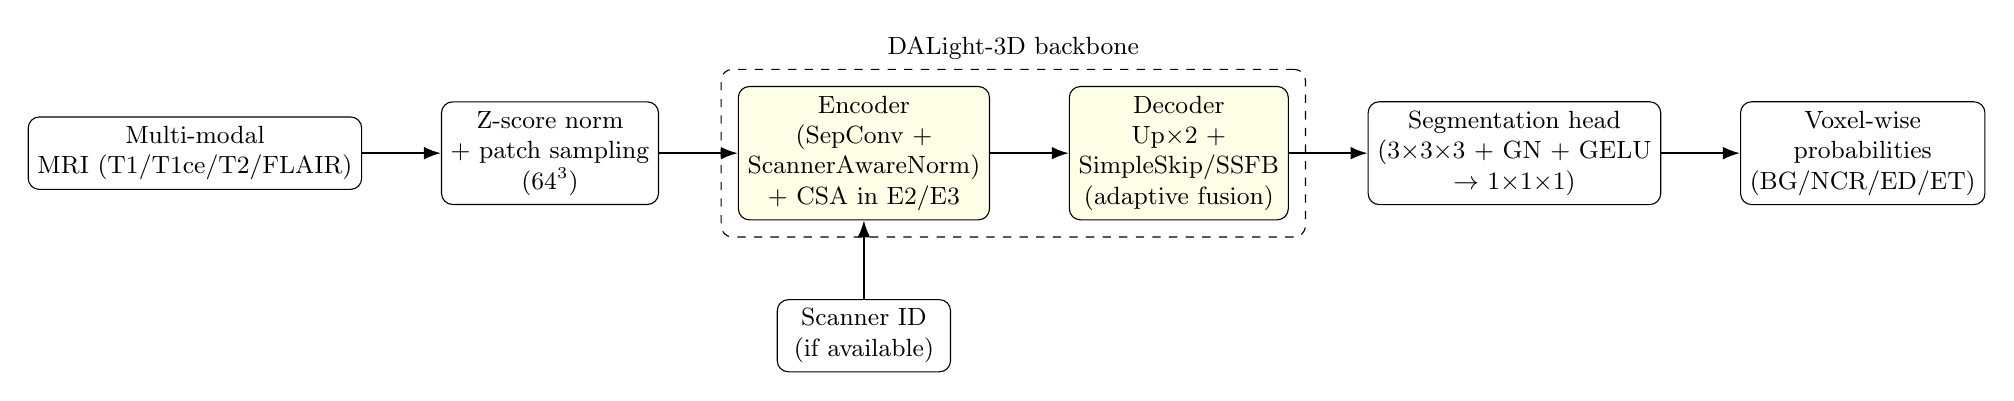
\begin{tikzpicture}[
  node distance=12mm and 10mm,
  box/.style={draw, rounded corners, align=center, minimum height=9mm, minimum width=22mm, font=\small},
  sbox/.style={draw, rounded corners, align=center, minimum height=8mm, minimum width=20mm, font=\small, fill=yellow!10},
  arr/.style={-Latex, line width=0.7pt},
]
  % Main flow
  \node[box] (in) {Multi-modal\\MRI (T1/T1ce/T2/FLAIR)};
  \node[box, right=of in] (prep) {Z-score norm\\+ patch sampling\\($64^3$)};
  \node[sbox, right=of prep] (enc) {Encoder\\(SepConv +\\ScannerAwareNorm)\\+ CSA in E2/E3};
  \node[sbox, right=of enc] (dec) {Decoder\\Up$\times2$ +\\SimpleSkip/SSFB\\(adaptive fusion)};
  \node[box, right=of dec] (head) {Segmentation head\\(3$\times$3$\times$3 + GN + GELU\\$\rightarrow$ 1$\times$1$\times$1)};
  \node[box, right=of head] (out) {Voxel-wise\\probabilities\\(BG/NCR/ED/ET)};

  \draw[arr] (in) -- (prep);
  \draw[arr] (prep) -- (enc);
  \draw[arr] (enc) -- (dec);
  \draw[arr] (dec) -- (head);
  \draw[arr] (head) -- (out);

  % Scanner conditioning side input
  \node[box, below=of enc, yshift=2mm] (sid) {Scanner ID\\(if available)};
  \draw[arr] (sid) -- (enc);

  % Group encoder/decoder
  \node[draw, dashed, rounded corners, fit=(enc) (dec), inner sep=6pt, label={[font=\small]above:DALight-3D backbone}] {};
\end{tikzpicture}
\caption{End-to-end DALight-3D pipeline (training/inference). Yellow blocks indicate the proposed architectural components.}
\label{fig:pipeline}
\end{figure*}

\begin{table}[t]
\centering
\caption{Feature dimensions in DALight-3D (input $64^3$, base $C_0=24$; evaluated configuration with bottleneck $432$, $\sim$2.2M parameters).}
\label{tab:dims}
\begin{tabular}{lcc}
\toprule
Stage & Resolution & Channels \\
\midrule
Input & $64^3$ & 4 \\
After Init & $64^3$ & 24 \\
E0, E1, E2, E3 & $64^3$, $32^3$, $16^3$, $8^3$ & 24, 48, 96, 432 \\
Bottleneck & $8^3$ & 432 \\
Decoder (D0, D1, D2) & $8^3$, $16^3$, $32^3$ & 432, 96, 48 \\
After final decoder & $64^3$ & 24 \\
Output & $64^3$ & 4 \\
\bottomrule
\end{tabular}
\end{table}

\begin{figure*}[t]
\centering
\includegraphics[width=\linewidth]{figures/architecture.png}
\caption{DALight-3D architecture used in this study. The first encoder block employs standard $3\times3\times3$ convolution, deeper encoder/decoder blocks use separable convolution, CSA is inserted in E2 and E3, the first decoder skip uses SimpleSkip, and the remaining skip paths use SSFB. Yellow denotes the emphasized design components, while blue/green blocks show the backbone encoder--decoder flow.}
\label{fig:arch}
\end{figure*}

Overall, DALight-3D preserves the beneficial inductive bias of 3D U-Net, but modifies the four most influential parts of the pipeline---convolution, normalization, context aggregation, and skip fusion---to obtain a more favorable efficiency--robustness trade-off.

%---------------------------------------------------------------------
\subsection{Encoder and Lightweight Feature Extraction}
\label{sec:encoder}

The encoder begins with an initial projection layer
\begin{equation}
\tilde{\mathbf{f}}^{(0)} = \mathrm{GELU}\big( \mathrm{GN}( \mathrm{Conv}_{3\times3\times3}(\mathbf{x}) ) \big),
\end{equation}
which maps the $M$ input modalities to $C_0$ channels. The first encoder feature map is then obtained as
\begin{equation}
\mathbf{f}^{(0)} = \mathrm{Block}^{(0)}(\tilde{\mathbf{f}}^{(0)}),
\end{equation}
where $\mathrm{Block}^{(0)}$ uses full $3\times3\times3$ convolution. For deeper levels,
\begin{equation}
\mathbf{f}^{(\ell)} = \mathrm{Block}^{(\ell)}\big( \mathrm{Downsample}(\mathbf{f}^{(\ell-1)}) \big), \qquad \ell = 1,2,3,
\end{equation}
where downsampling is implemented by a strided $3\times3\times3$ convolution with stride $2$. This structure yields progressively coarser but semantically richer features, with CSA appended only at the deeper levels.

%---------------------------------------------------------------------
\subsection{LightweightBlock}
\label{sec:lightweightblock}

The \textbf{LightweightBlock} is the main residual unit of DALight-3D. Given an input tensor $\mathbf{h} \in \mathbb{R}^{C_{\mathrm{in}} \times D \times H \times W}$, the block applies two convolution--normalization transformations followed by channel recalibration:
\begin{equation}
\mathbf{z} = \mathrm{SE}\!\Big( \mathrm{Norm}_2\big( \mathrm{Conv}_2( \phi( \mathrm{Norm}_1( \mathrm{Conv}_1(\mathbf{h}) ) ) ) \big) \Big),
\end{equation}
where $\phi$ denotes GELU, $\mathrm{Norm}_1$ and $\mathrm{Norm}_2$ denote ScannerAwareNorm (or GroupNorm when scanner conditioning is unavailable), and $\mathrm{Conv}_i$ is standard convolution in E0 and SepConv in E1--E3. For encoder stages E2 and E3, contextual refinement is added by
\begin{equation}
\mathbf{z} \leftarrow \mathbf{z} + \mathrm{CrossSliceAttn}(\mathbf{z}).
\end{equation}
A residual projection then produces the block output:
\begin{equation}
\mathbf{o} = \phi\big(\mathbf{z} + \mathrm{Proj}(\mathbf{h})\big),
\end{equation}
where $\mathrm{Proj}$ is identity when shapes match and a $1\times1\times1$ projection otherwise.

%---------------------------------------------------------------------
\subsection{Separable 3D Convolution (SepConv)}
\label{sec:sepconv}

A standard 3D convolution requires $\mathcal{O}(C_{\mathrm{in}} C_{\mathrm{out}} k^3)$ parameters, which rapidly increases memory and computation as the feature width grows. DALight-3D therefore uses depthwise separable 3D convolution~\cite{howard2017mobilenets} in the deeper encoder and decoder blocks. Given an input feature map $\mathbf{u}$, SepConv is written as
\begin{equation}
\mathbf{v} = \mathcal{W}_{\mathrm{dw}} \ast \mathbf{u},
\end{equation}
\begin{equation}
\mathbf{y} = \mathcal{W}_{\mathrm{pw}} \ast \mathbf{v},
\end{equation}
where $\mathcal{W}_{\mathrm{dw}}$ performs channel-wise spatial filtering and $\mathcal{W}_{\mathrm{pw}}$ performs $1\times1\times1$ channel mixing. The corresponding parameter cost becomes $C_{\mathrm{in}}k^3 + C_{\mathrm{in}}C_{\mathrm{out}}$, which is substantially lower than that of a full convolution while preserving local volumetric receptive fields.

%---------------------------------------------------------------------
\subsection{Scanner-Aware Normalization (ScannerAwareNorm)}
\label{sec:scannorm}

A recurring challenge in multi-site MRI is that feature statistics can shift across scanners and acquisition protocols. To account for this explicitly, DALight-3D introduces \textbf{ScannerAwareNorm}, a scanner-conditioned extension of Group Normalization~\cite{wu2018groupnorm}. For a feature tensor $\mathbf{x}$, we first compute
\begin{equation}
\hat{\mathbf{x}} = \mathrm{GN}(\mathbf{x}),
\end{equation}
then modulate the normalized activations using scanner-conditioned affine parameters:
\begin{equation}
\mathbf{y} = \gamma_s \odot \hat{\mathbf{x}} + \beta_s,
\end{equation}
where $\gamma_s = \mathbf{E}_{\gamma}(s)$ and $\beta_s = \mathbf{E}_{\beta}(s)$ are learnable embeddings indexed by scanner identity $s$. When scanner information is unavailable, the module falls back to learned default affine parameters. In contrast to generic normalization alone, this mechanism allows the network to adapt internal feature statistics to acquisition-specific variation without adding a separate domain adaptation branch.

%---------------------------------------------------------------------
\subsection{Cross-Slice Attention (CSA)}
\label{sec:csa}

Although 3D convolution captures local neighborhoods well, it does not explicitly model long-range dependencies across distant slices. DALight-3D therefore employs \textbf{Cross-Slice Attention (CSA)} in the deeper encoder stages, where semantic abstraction is strongest. Given
\begin{equation}
\mathbf{x} \in \mathbb{R}^{B \times C \times D \times H \times W},
\end{equation}
we first pool over the in-plane dimensions to obtain a depth-wise descriptor
\begin{equation}
\mathbf{p} = \mathrm{Pool}_{H,W}(\mathbf{x}) \in \mathbb{R}^{B \times C \times D}.
\end{equation}
Low-rank query, key, and value projections are then computed as
\begin{equation}
Q = W_q \mathbf{p}, \qquad K = W_k \mathbf{p}, \qquad V = W_v \mathbf{p}.
\end{equation}
The slice-attention matrix is
\begin{equation}
A = \mathrm{softmax}\left( \frac{Q^\top K}{\sqrt{d}} \right),
\end{equation}
and the refined output is given by
\begin{equation}
\mathrm{CSA}(\mathbf{x}) = \mathbf{x} + \mathrm{Broadcast}(W_o V A).
\end{equation}
Because attention is computed along the slice axis rather than across all voxels, the effective complexity is reduced from $O((DHW)^2)$ to $O(D^2)$.

%---------------------------------------------------------------------
\subsection{Decoder and Multi-scale Feature Fusion}
\label{sec:decoder}

The decoder reconstructs the segmentation map progressively through transposed-convolution upsampling. At each resolution level, the upsampled decoder representation is fused with its corresponding encoder feature map and then refined by a LightweightBlock without CSA. The first skip path, nearest to the bottleneck, uses a simple concatenation-based fusion to stabilize optimization. The remaining skip paths use the proposed SSFB module to allow adaptive interaction between encoder detail and decoder semantics. When exact spatial alignment is not available, trilinear interpolation is used before fusion.

%---------------------------------------------------------------------
\subsection{Skip and Spatial Feature Blend (SSFB)}
\label{sec:ssfb}

The \textbf{Skip and Spatial Feature Blend (SSFB)} module is designed to improve skip fusion beyond naive concatenation. Let $\mathbf{f}_{\mathrm{dec}}$ and $\mathbf{f}_{\mathrm{enc}}$ denote the aligned decoder and encoder feature maps. SSFB combines two complementary pathways.

\paragraph{Low-rank attention pathway.}
A low-rank cross-attention operation computes
\begin{equation}
\mathbf{o}_{\mathrm{attn}} = W_{\mathrm{out}}(VA),
\end{equation}
where $A$ is formed from low-rank query and key projections of the decoder and encoder features.

\paragraph{Channel-gating pathway.}
A channel-reweighting branch computes
\[
\mathbf{o}_{\mathrm{gate}} = \mathbf{f}_{\mathrm{enc}} \odot \sigma\big( \mathrm{MLP}( [\mathrm{GAP}(\mathbf{f}_{\mathrm{dec}}); \mathrm{GAP}(\mathbf{f}_{\mathrm{enc}})] ) \big),
\]
where $\mathrm{GAP}$ denotes global average pooling and $\sigma$ is the sigmoid nonlinearity.

The two branches are blended through a learnable scalar:
\begin{equation}
\mathbf{m} = \alpha \, \mathbf{o}_{\mathrm{attn}} + (1-\alpha) \, \mathbf{o}_{\mathrm{gate}},
\end{equation}
where $\alpha \in (0,1)$ is optimized during training. The final SSFB output is
\begin{equation}
\mathrm{SSFB}(\mathbf{f}_{\mathrm{dec}}, \mathbf{f}_{\mathrm{enc}}) = \phi\!\left(\mathrm{GN}\!\left(\mathrm{Conv}_{3\times3\times3}([\mathbf{f}_{\mathrm{dec}};\mathbf{m}])\right)\right).
\end{equation}
This formulation allows the decoder to exploit both similarity-aware interaction and channel-selective gating when integrating encoder information.

%---------------------------------------------------------------------
\subsection{Segmentation Head}
\label{sec:head}

The final decoder representation is converted to voxel-wise logits through a lightweight segmentation head:
\begin{equation}
\mathbf{z} = \mathrm{Conv}_{1\times1\times1}\big(\phi(\mathrm{GN}(\mathrm{Conv}_{3\times3\times3}(\mathbf{f}_{\mathrm{dec}})))\big).
\end{equation}
A softmax layer then produces the class-probability volume $\mathbf{p}$. This head retains local refinement capacity while keeping the prediction stage compact.

%---------------------------------------------------------------------
\subsection{Qualitative Segmentation Visualization}
\label{sec:qualitative}

To complement the quantitative analysis, we visualize representative tumor-containing slices with ground-truth and predicted subregion overlays. As in recent BraTS-style studies, these qualitative results help assess whether the model captures the morphology and boundaries of NCR, ED, and ET consistently across cases.

\begin{figure}[t]
\centering
\includegraphics[width=\linewidth]{figures/qualitative_segmentation.png}
\caption{Qualitative segmentation on representative tumor-containing slices. Ground-truth and DALight-3D predictions are shown for the NCR, ED, and ET subregions.}
\label{fig:qualitative-seg}
\end{figure}

\subsection{Model Decision Process: Confidence and Uncertainty}
\label{sec:decision}

To improve interpretability, we further visualize the model's confidence and uncertainty. Confidence is defined as the maximum class probability at each voxel, whereas uncertainty is measured as Shannon entropy over the predicted class distribution. High-confidence regions generally correspond to stable tissue assignments, while elevated entropy tends to occur near ambiguous tumor boundaries and transitional regions.

\begin{figure}[t]
\centering
\includegraphics[width=\linewidth]{figures/decision_process.png}
\caption{Model decision process on representative tumor-containing cases. From left to right: predicted overlay, confidence map (maximum probability), and uncertainty map (entropy).}
\label{fig:decision-process}
\end{figure}

\vspace{-2mm}
\subsection{Training Objective}
\label{sec:loss}

The training objective combines overlap-sensitive Dice optimization with voxel-wise probabilistic supervision:
\begin{equation}
\mathcal{L} = \lambda_{\mathrm{Dice}} \mathcal{L}_{\mathrm{Dice}}(\mathbf{p}, \mathbf{y}) + \lambda_{\mathrm{CE}} \mathcal{L}_{\mathrm{CE}}(\mathbf{p}, \mathbf{y}),
\end{equation}
with
\begin{equation}
\lambda_{\mathrm{Dice}}=1, \qquad \lambda_{\mathrm{CE}}=0.5.
\end{equation}
Let $\mathcal{T}=\{\text{NCR},\text{ED},\text{ET}\}$ denote the tumor classes and let $y_c(v)$ be the one-hot target for class $c$ at voxel $v$. The Dice term is defined as
\begin{equation}
\mathcal{L}_{\mathrm{Dice}} = 1 - \frac{1}{|\mathcal{T}|} \sum_{c \in \mathcal{T}} \frac{2\sum_{v \in \Omega} p_c(v) y_c(v) + \epsilon}{\sum_{v \in \Omega} p_c(v) + \sum_{v \in \Omega} y_c(v) + \epsilon},
\end{equation}
and the cross-entropy term is
\begin{equation}
\mathcal{L}_{\mathrm{CE}} = -\frac{1}{|\Omega|} \sum_{v \in \Omega} \sum_{c=1}^{K} y_c(v) \log p_c(v).
\end{equation}
This hybrid objective is well suited to brain tumor segmentation because it simultaneously addresses severe class imbalance and encourages calibrated voxel-wise discrimination.

%==============================================================================
\section{Evaluation}
\label{sec:eval}
%==============================================================================

\subsection{Experimental Setup}
\label{sec:experimental_setup}

All experiments were conducted on a local workstation running macOS 26.3.1 with an Apple M3 Pro processor and 36\,GB unified memory. Model development, training, evaluation, and figure generation were performed in a Python/PyTorch environment, with the reported comparative runs executed on CPU to ensure a consistent and reproducible setup across the proposed model and all baselines.

\subsection{Dataset and Preprocessing}
\label{sec:dataset}

Experiments are conducted on the Medical Segmentation Decathlon Task01\_BrainTumour dataset~\cite{simpson2019msd}, a BraTS-derived multi-modal MRI benchmark containing T1, T1ce, T2, and FLAIR volumes with voxel-wise annotations for background (BG), necrotic/non-enhancing tumor core (NCR), peritumoral edema (ED), and enhancing tumor (ET). We follow the official training/validation partition. Each case is normalized independently using z-score normalization, and training is performed on tumor-centered $64^3$ patches. Random flips and light intensity perturbations are applied online for augmentation. Scanner identifiers are used as conditioning input for ScannerAwareNorm when available.

\subsection{Implementation and Training Protocol}
\label{sec:implementation}

All models are implemented in PyTorch and trained under matched settings to ensure a controlled comparison. We use AdamW with learning rate $5\times10^{-5}$, a cosine annealing scheduler, and the hybrid Dice plus cross-entropy objective with $\lambda_{\mathrm{Dice}}=1$ and $\lambda_{\mathrm{CE}}=0.5$. Training is run for 10 epochs with batch size 1 and validation every 2 epochs. Mixed precision is disabled to avoid numerical instability. The proposed DALight-3D uses base width $C_0=24$, bottleneck width 432, and SSFB rank 8, resulting in approximately 2.22M trainable parameters. The comparison models---standard 3D U-Net~\cite{cicek20163dunet}, Attention U-Net~\cite{oktay2018attentionunet}, and Residual 3D U-Net~\cite{he2016resnet}---share the same training protocol and base width so that the observed differences primarily reflect architectural design.

\subsection{Component-Wise Ablation Protocol}
\label{sec:ablation_protocol}

To isolate the contribution of each proposed module, we define a component-wise ablation protocol in which one design element is removed at a time while all other training and architectural settings are kept fixed. This design is intended to separate the effect of efficiency-oriented operators from that of scanner-aware normalization, contextual aggregation, and adaptive skip fusion. The ablation variants considered in this study are summarized in Table~\ref{tab:ablation_protocol}. Under this protocol, the full DALight-3D model serves as the reference configuration, and each ablation removes a single proposed component while preserving the same input resolution, optimization settings, and evaluation metrics.

\begin{table}[t]
\centering
\caption{Component-wise ablation protocol for DALight-3D. Each variant removes one proposed component while preserving the remaining architecture and training setup.}
\label{tab:ablation_protocol}
\begin{tabular}{ll}
\toprule
Variant & Modification relative to full DALight-3D \\
\midrule
Full model & All proposed components enabled \\
w/o SepConv & Replace deeper separable convolutions with standard 3D convolutions \\
w/o ScannerAwareNorm & Replace scanner-conditioned normalization with GroupNorm \\
w/o CSA & Remove cross-slice attention from the deep encoder stages \\
w/o SSFB & Replace SSFB with simple skip fusion throughout decoding \\
\bottomrule
\end{tabular}
\end{table}

%---------------------------------------------------------------------
\subsection{Results}
\label{sec:results}

\subsubsection{Comparison with Baselines}

Table~\ref{tab:comparison} presents the primary quantitative comparison across all evaluated models. The table reports three complementary quantities: mean Dice as the principal segmentation metric, total trainable parameters as a measure of model complexity, and Dice per million parameters as a compact indicator of parameter efficiency. DALight-3D attains the highest mean Dice (0.657) while also being the most compact model in the study (2.22M parameters). The strongest baseline, Residual 3D U-Net, reaches 0.652 Dice with 3.20M parameters, whereas the standard and attention-based 3D U-Nets obtain 0.612 and 0.565 Dice, respectively. Relative to the strongest baseline, the proposed model improves mean Dice by 0.005 while reducing parameters by approximately 31\%; relative to the standard and attention baselines, the Dice gains increase to 0.045 and 0.092, respectively, again with a markedly smaller footprint. The best Dice-per-million-parameters value further confirms that the proposed model is not simply smaller, but more effective per unit capacity.

\begin{table}[t]
\centering
\caption{Comparison of DALight-3D against CNN baselines on Task01\_BrainTumour under identical 10-epoch training. Best mean Dice is shown in \textbf{bold}; best Dice per million parameters is shown in \emph{italic}.}
\label{tab:comparison}
\begin{tabular}{lccc}
\toprule
Method & Mean Dice $\uparrow$ & Params (M) & Dice/M \\
\midrule
Standard 3D U-Net & 0.612 & 3.15 & 0.19 \\
Attention U-Net & 0.565 & 3.17 & 0.18 \\
Residual 3D U-Net & 0.652 & 3.20 & 0.20 \\
\textbf{DALight-3D (Ours)} & \textbf{0.657} & \textbf{2.22} & \emph{0.30} \\
\bottomrule
\end{tabular}
\end{table}

Figure~\ref{fig:dice_params} and Figure~\ref{fig:compare_dice_params_bar} visualize this same relationship from two complementary perspectives. Figure~\ref{fig:dice_params} is a trade-off scatter plot in which the horizontal axis represents model size and the vertical axis represents segmentation quality; the most desirable region is therefore the upper-left corner, corresponding to high accuracy and low complexity. DALight-3D occupies precisely this region, whereas all baselines are shifted to the right, indicating higher parameter count, without surpassing the proposed model in Dice. Figure~\ref{fig:compare_dice_params_bar} presents the same evidence in side-by-side bar form, making the numerical gap easier to compare visually. Taken together, these two figures show that the proposed method improves the operating point rather than merely shifting the balance between accuracy and efficiency.

\begin{figure}[t]
\centering
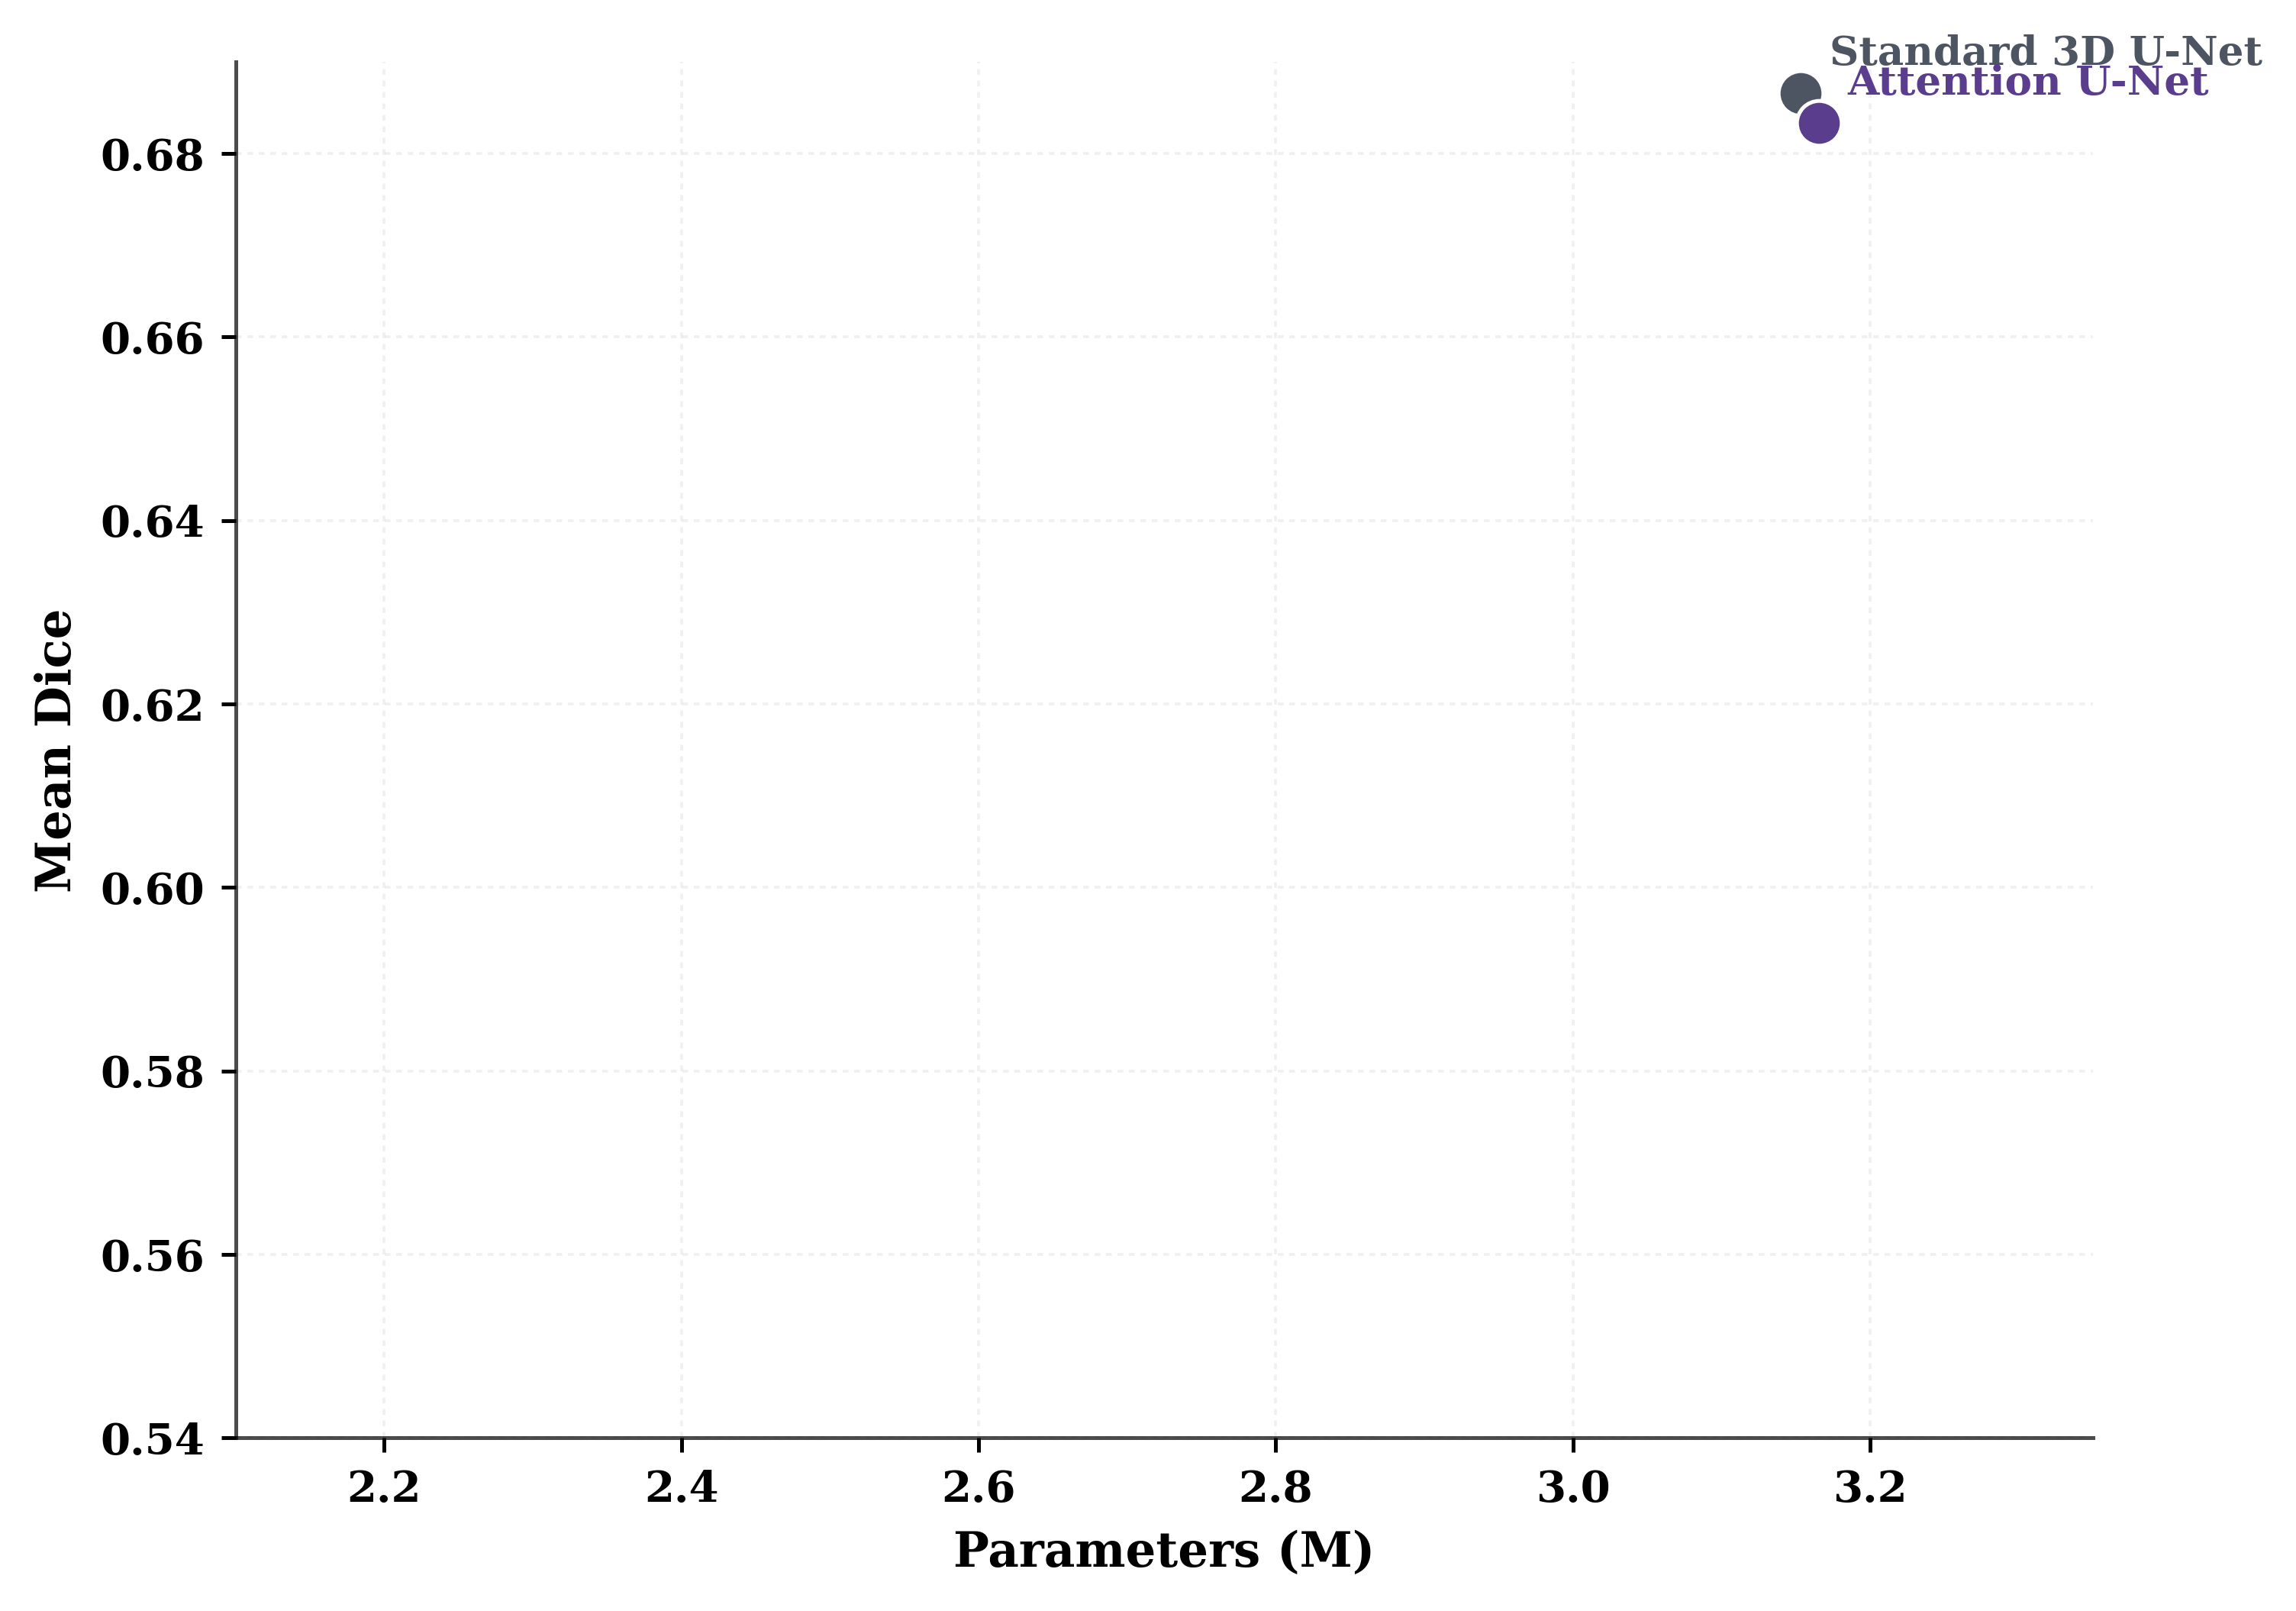
\includegraphics[width=\linewidth]{figures/eval/dice_params_tradeoff_scatter.png}
\caption{Accuracy--efficiency trade-off measured by mean Dice and parameter count (millions). DALight-3D occupies the upper-left region, indicating the most favorable balance of segmentation quality and model compactness among the compared methods.}
\label{fig:dice_params}
\end{figure}

\begin{figure}[t]
\centering
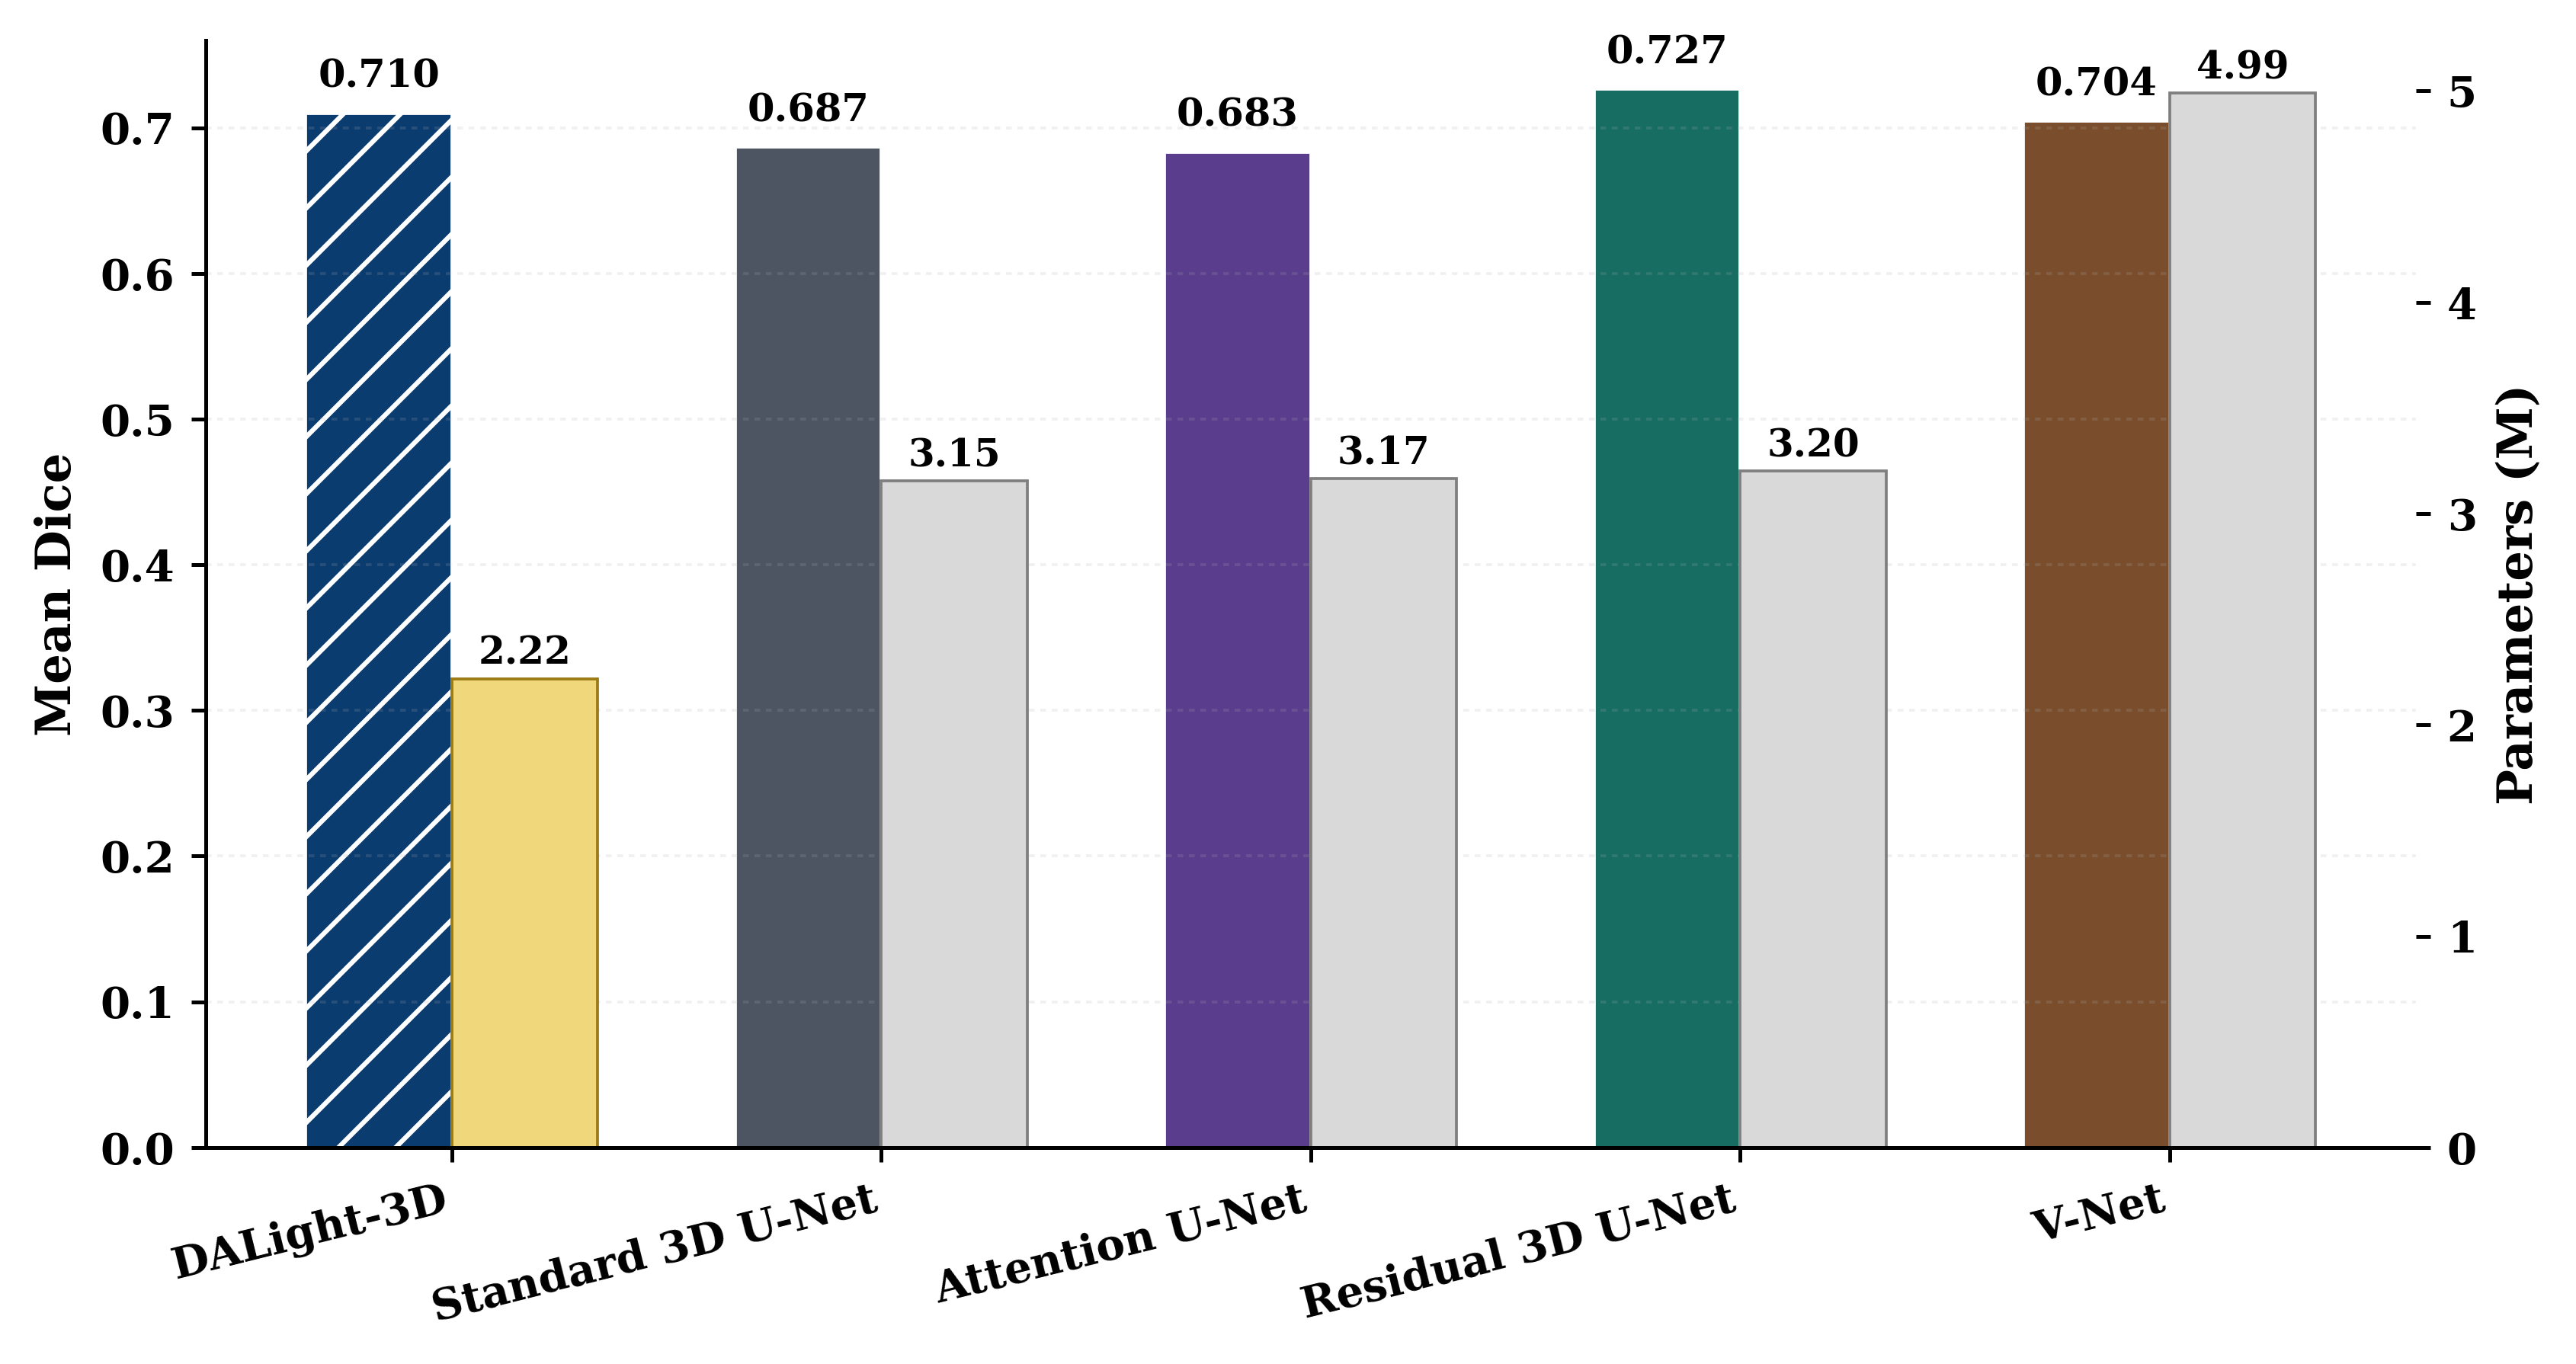
\includegraphics[width=\linewidth]{figures/eval/compare_dice_params_bar.png}
\caption{Side-by-side comparison of mean Dice and parameter count across DALight-3D and the baseline models, highlighting that the proposed method achieves both the best Dice and the lowest parameter count.}
\label{fig:compare_dice_params_bar}
\end{figure}

\subsubsection{Learning Curves}

The learning-curve analysis is used to assess whether the proposed gains arise from stable optimization rather than isolated endpoint fluctuations. Figure~\ref{fig:curves} jointly reports DALight-3D training loss and validation Dice over the 10-epoch schedule. The loss decreases consistently while validation Dice improves throughout training, indicating that optimization remains stable and that the model continues to extract useful structure from the data over the observed epoch range. The absence of a late-stage collapse or abrupt divergence suggests that the proposed lightweight design does not compromise trainability.

Figure~\ref{fig:compare_val_dice} compares validation Dice trajectories across DALight-3D and the baseline models. This figure represents how rapidly and how consistently each model translates training into validation-set improvement. DALight-3D remains competitive throughout training and finishes with the highest final validation Dice, which strengthens the conclusion that its advantage is not confined to a transient epoch. Figure~\ref{fig:compare_train_loss} complements this view by plotting training loss for all models. The loss curves show that the proposed method achieves competitive optimization behavior despite its lower parameter budget, indicating that the observed Dice gains are not the result of over-parameterization but of more effective feature utilization.

\begin{figure}[t]
\centering
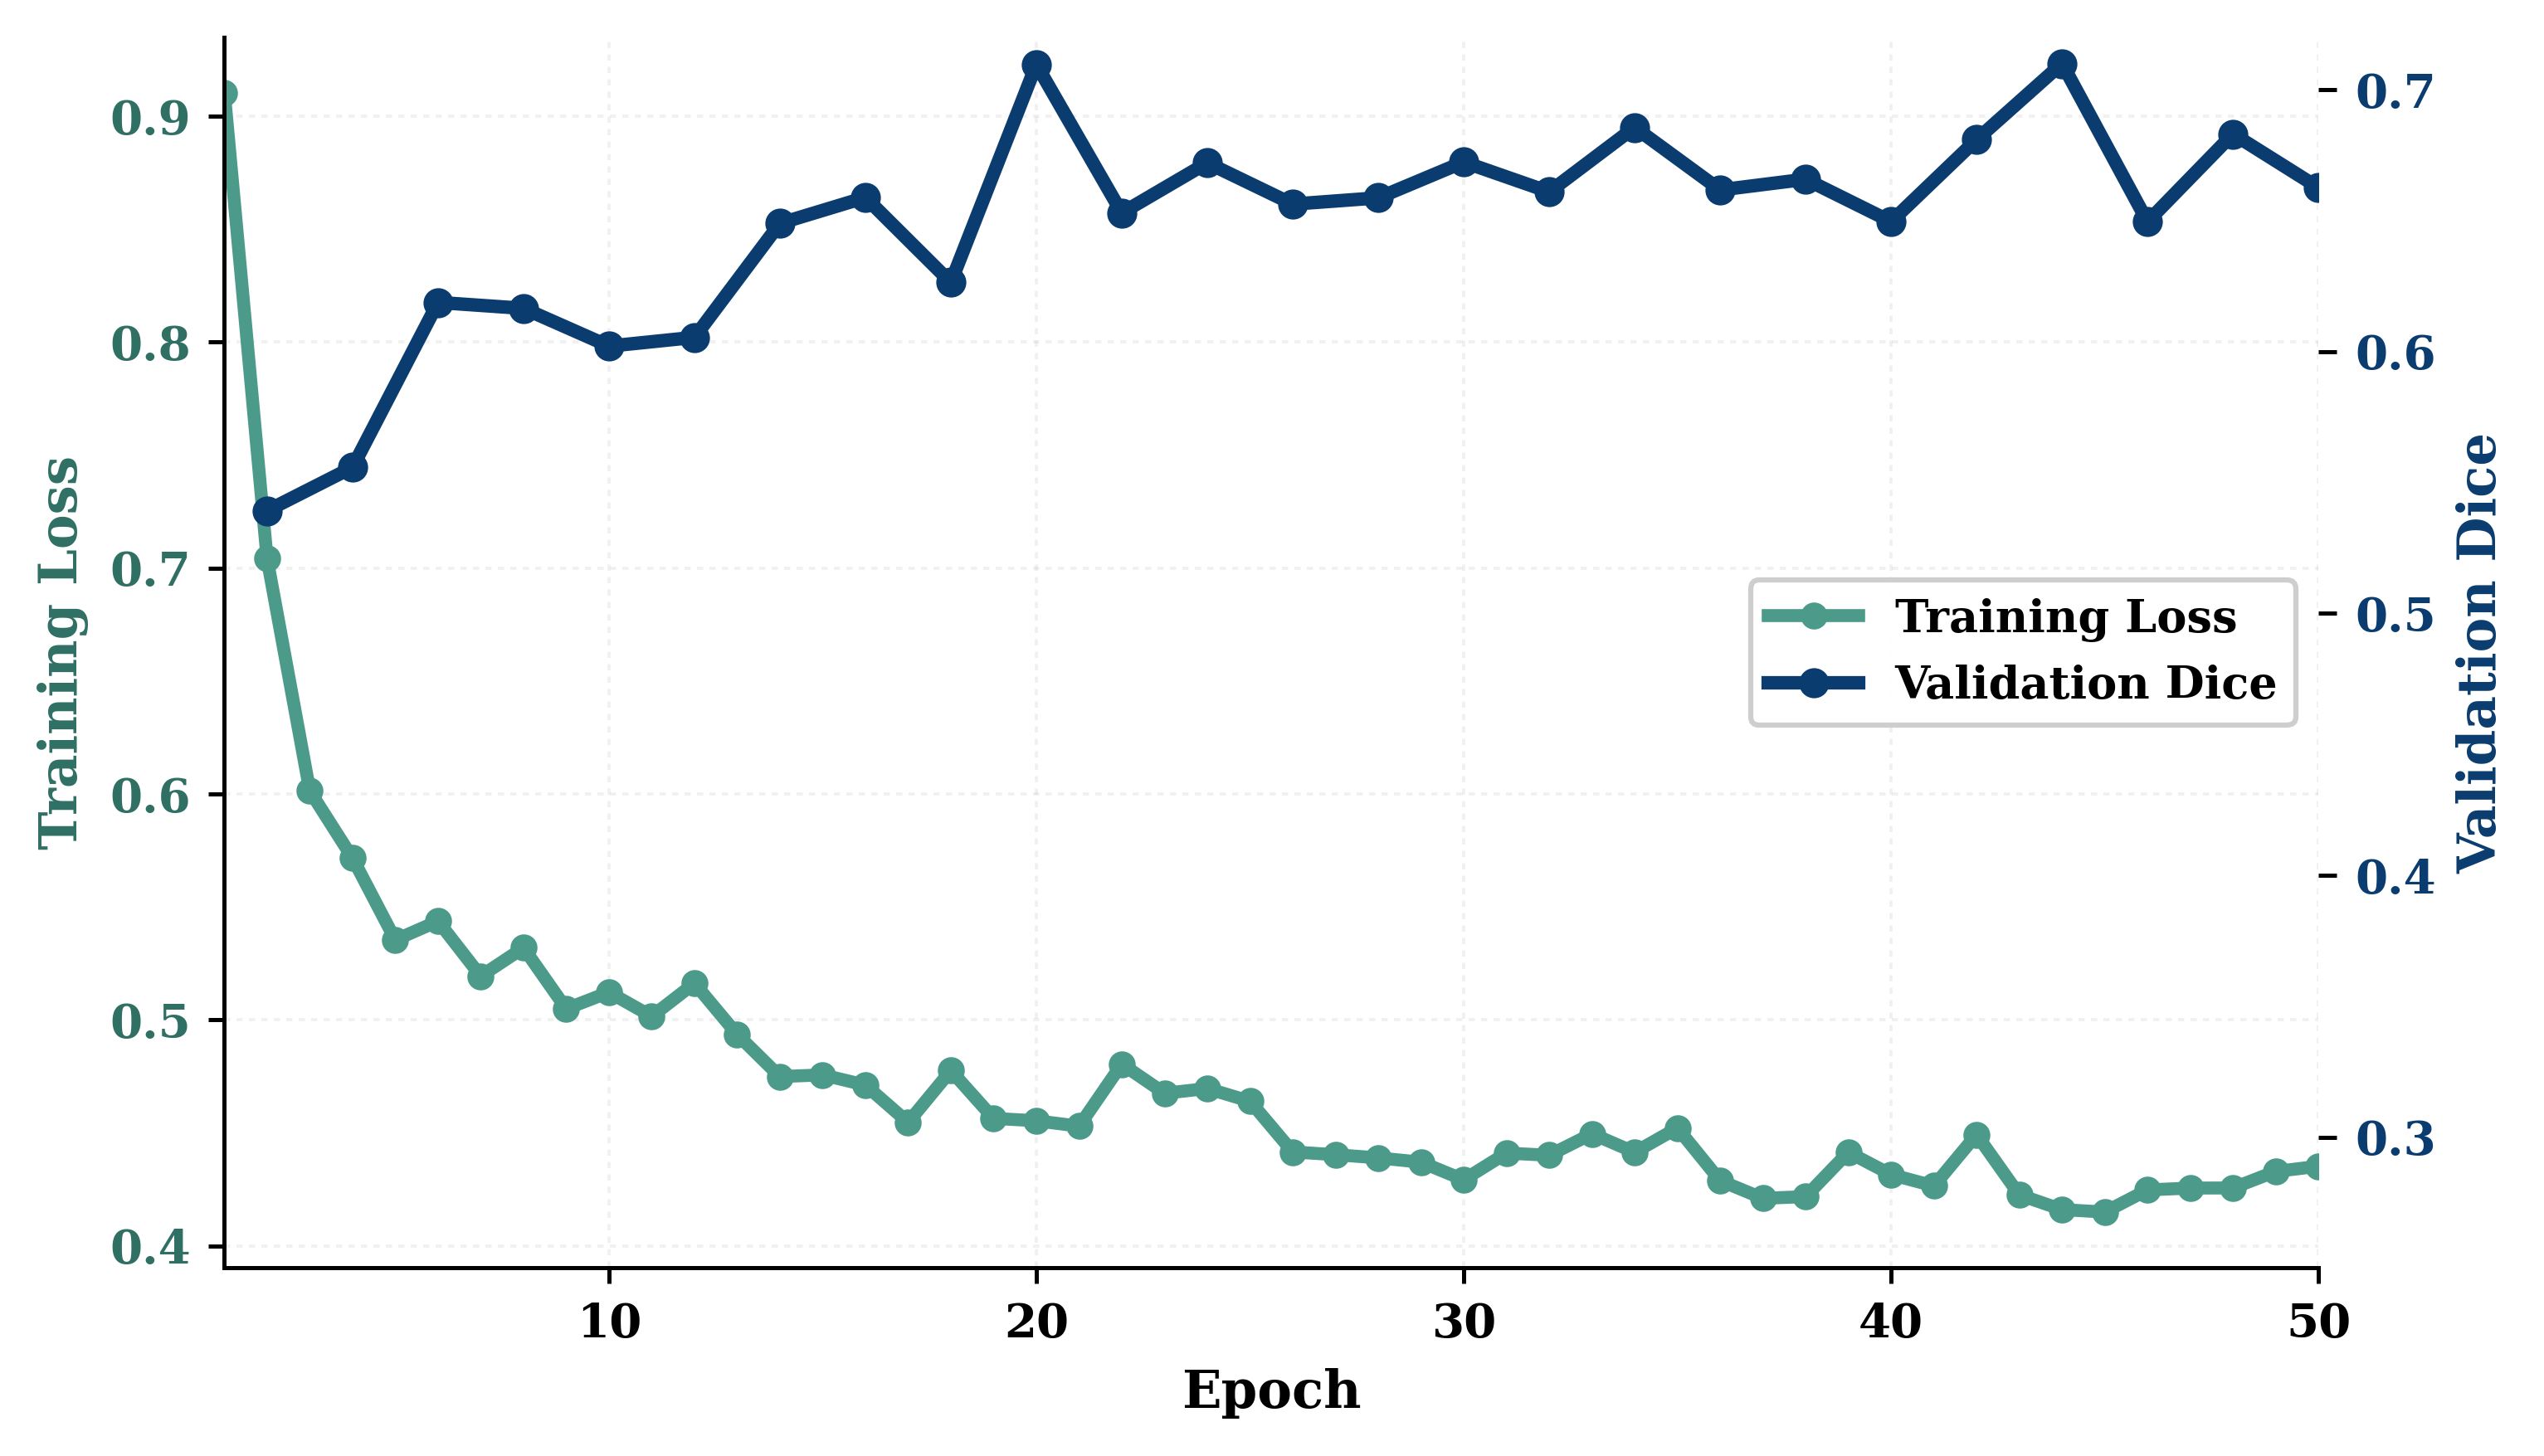
\includegraphics[width=\linewidth]{figures/eval/loss_and_dice.png}
\caption{Training dynamics of DALight-3D over 10 epochs, showing decreasing loss and improving validation Dice.}
\label{fig:curves}
\end{figure}

\begin{figure}[t]
\centering
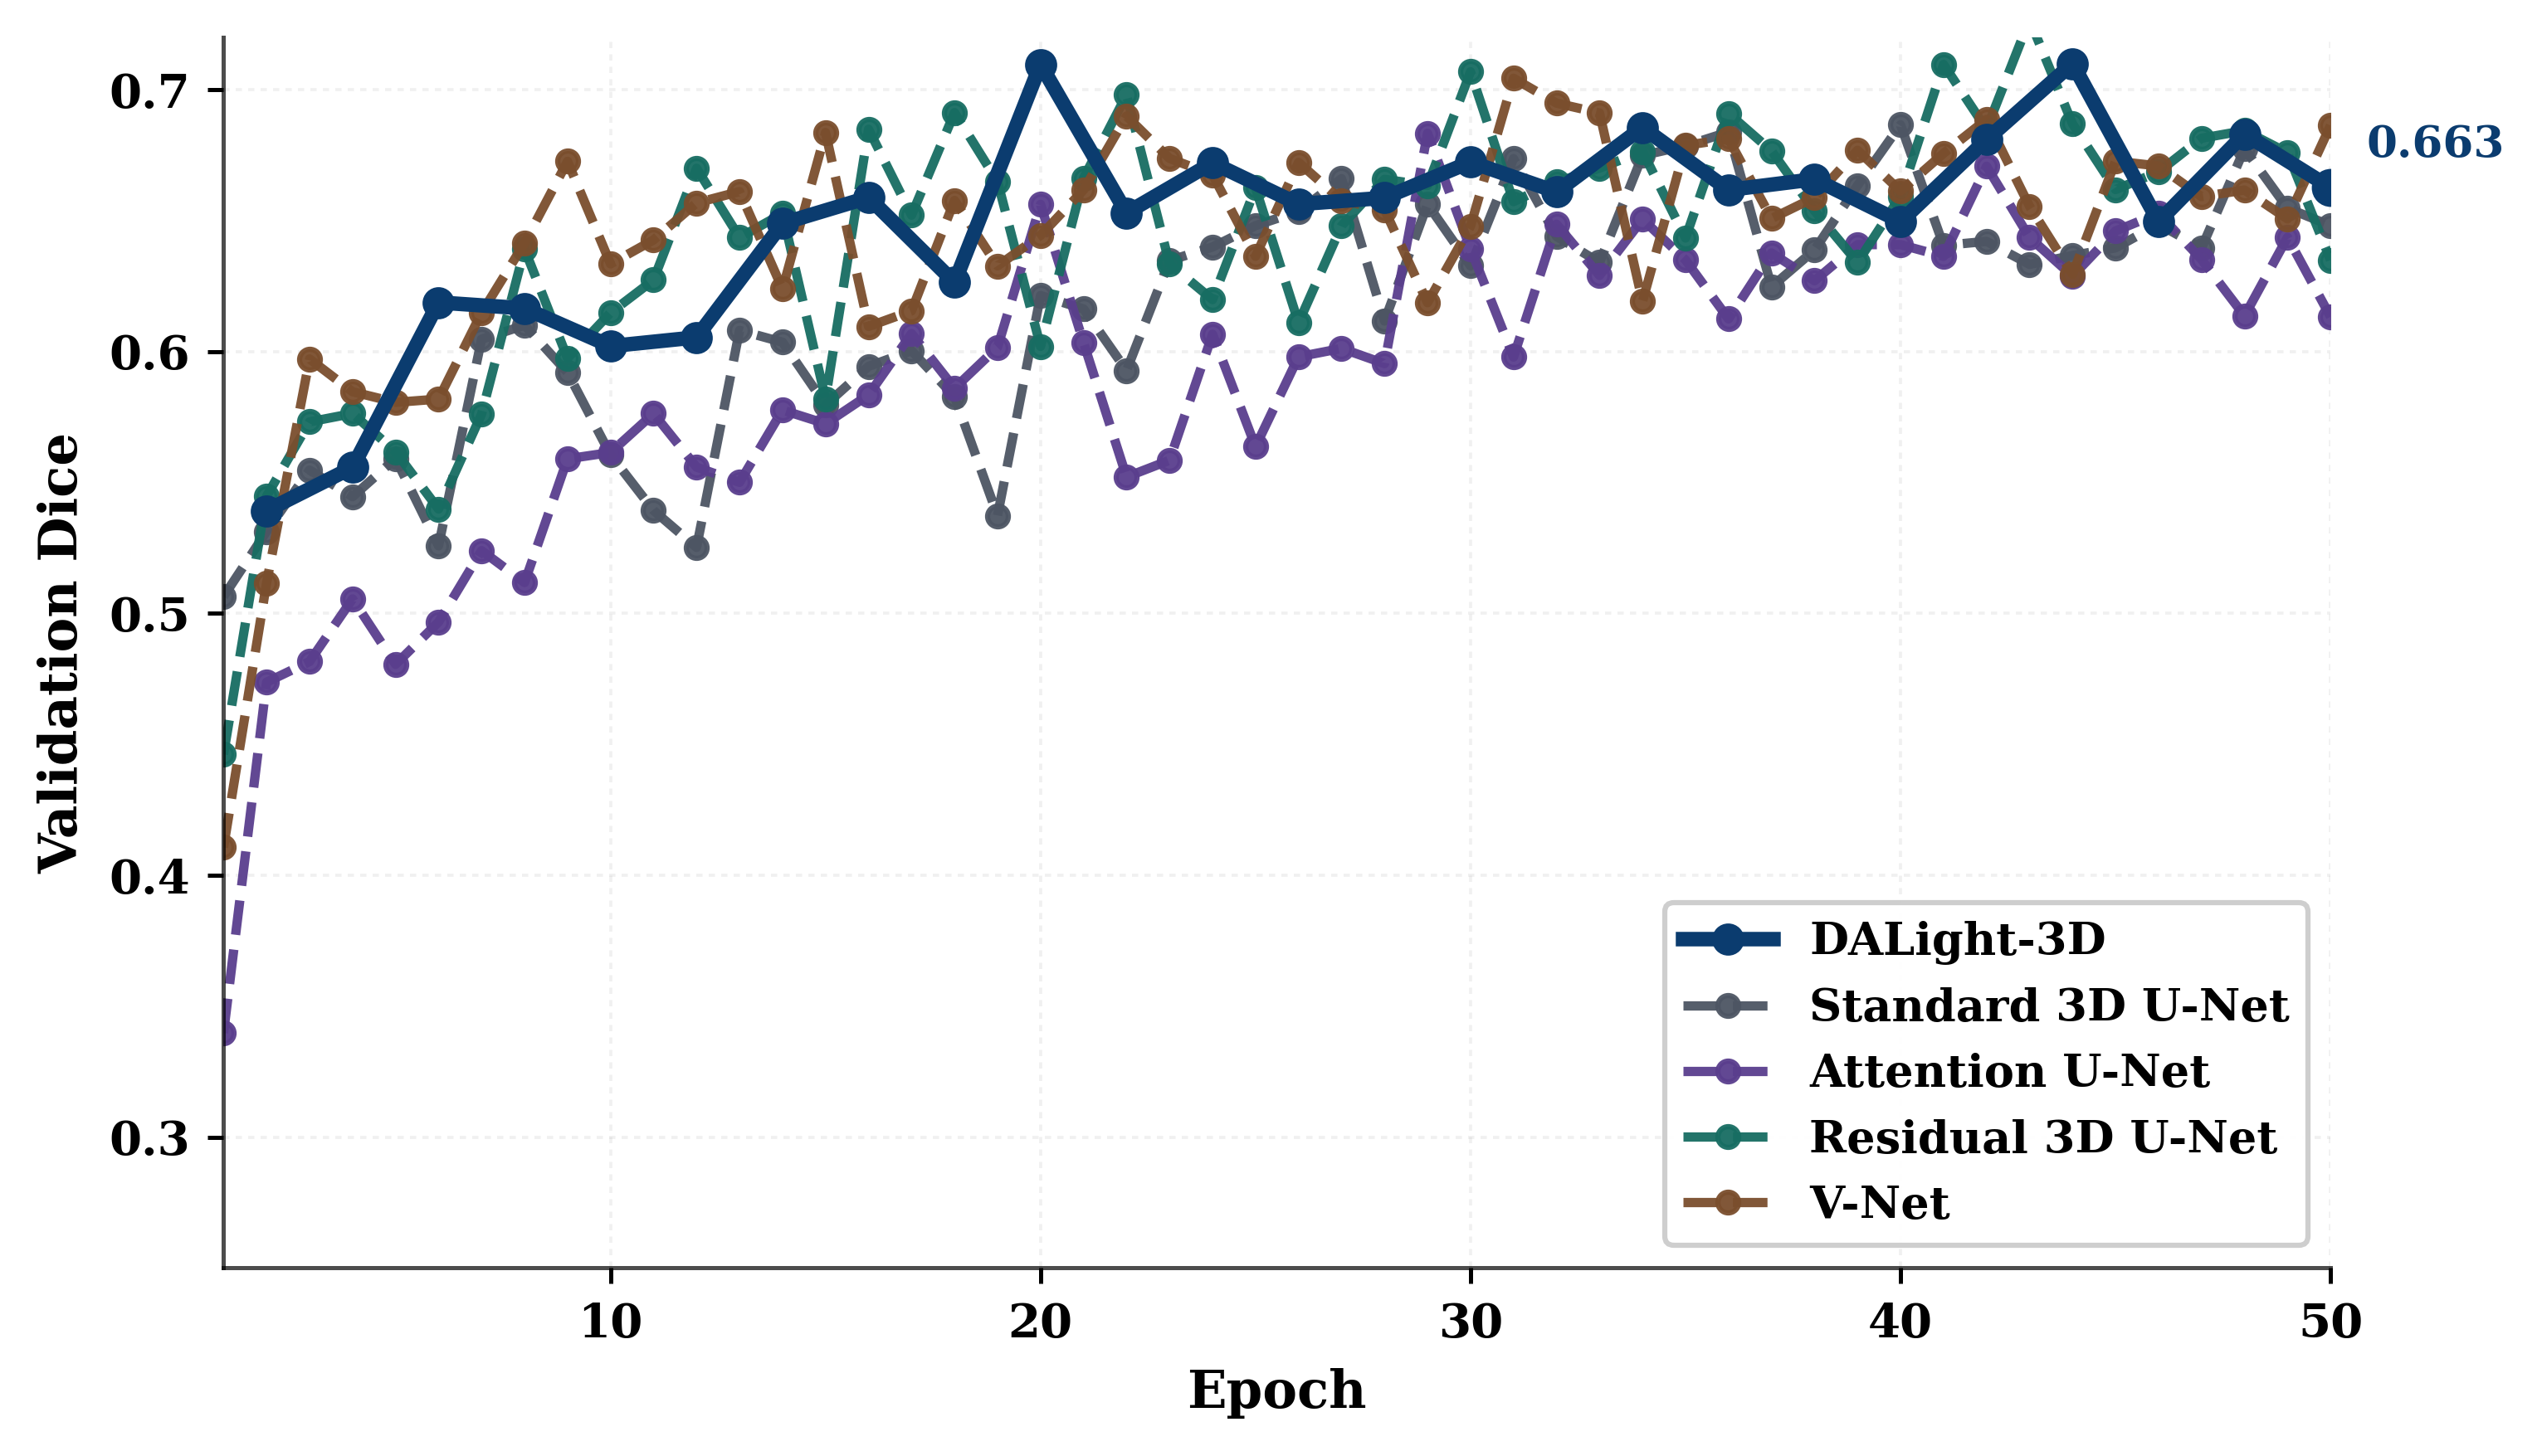
\includegraphics[width=\linewidth]{figures/eval/compare_val_dice.png}
\caption{Validation Dice trajectories for DALight-3D and the baseline models under identical training settings.}
\label{fig:compare_val_dice}
\end{figure}

\begin{figure}[t]
\centering
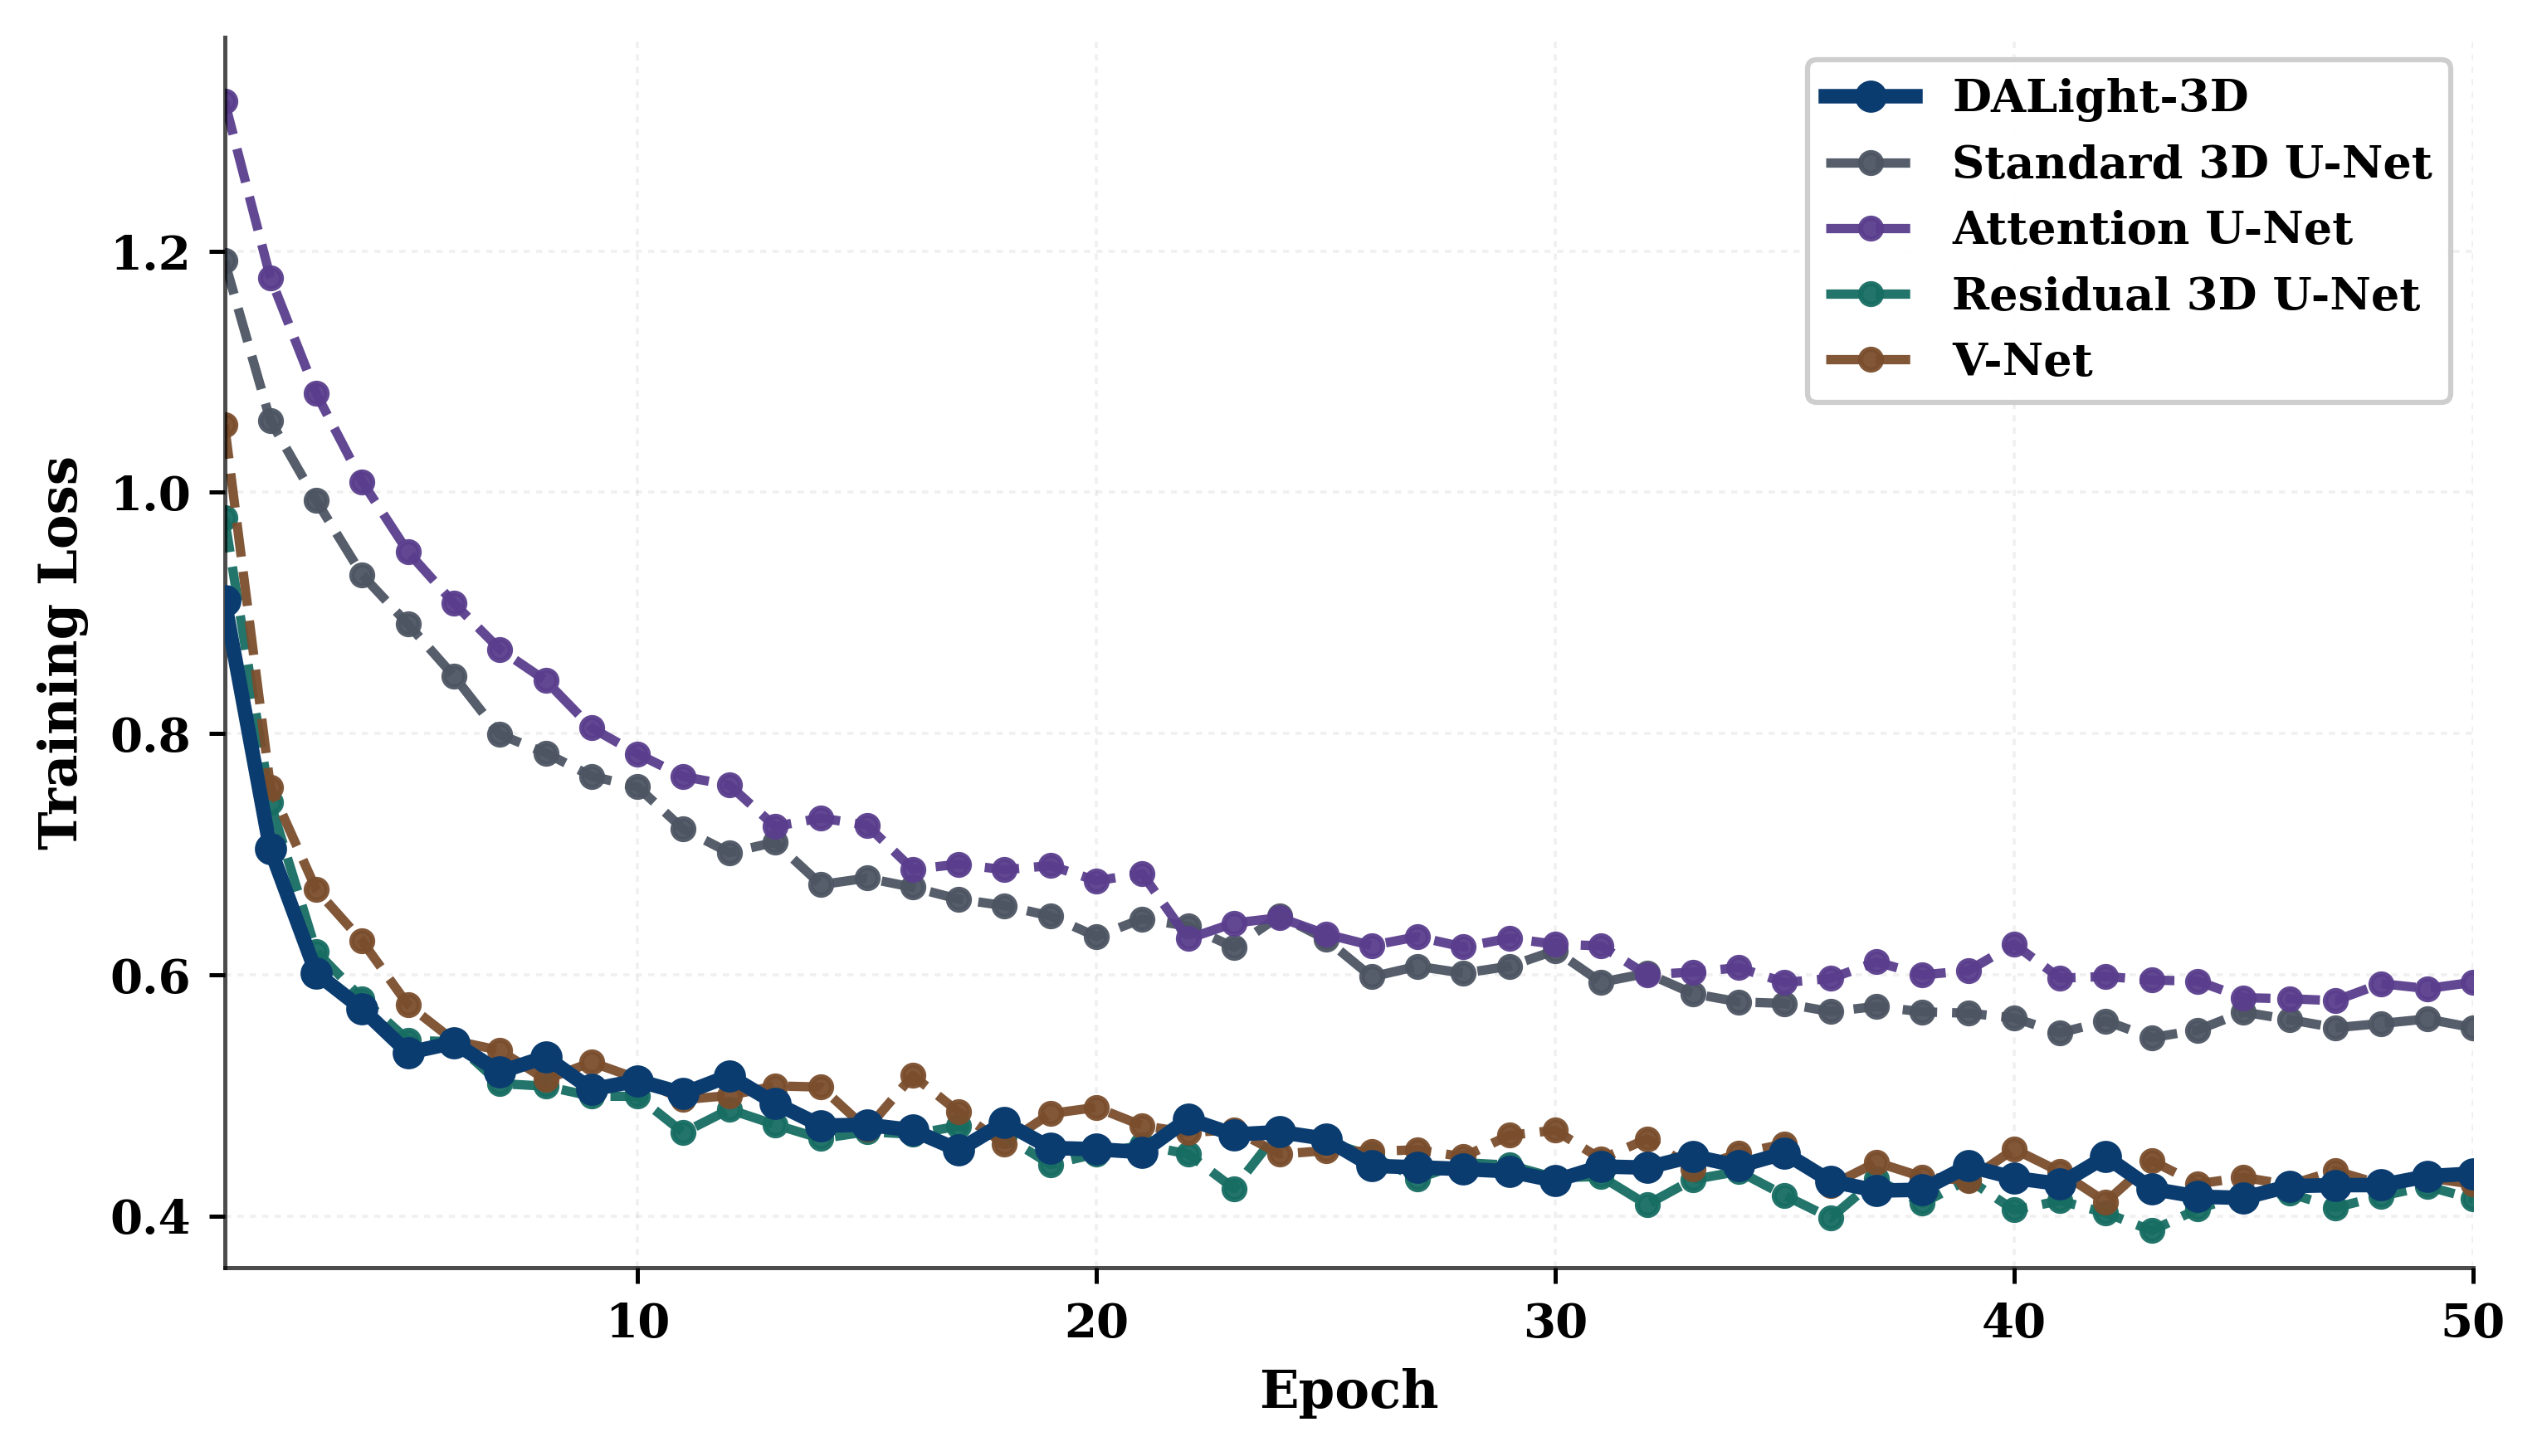
\includegraphics[width=\linewidth]{figures/eval/compare_train_loss.png}
\caption{Training loss trajectories for DALight-3D and the baseline models under identical training settings.}
\label{fig:compare_train_loss}
\end{figure}

\subsubsection{Per-Class Performance and Confusion Matrix}

The aggregate Dice score does not reveal which anatomical subregions are easier or harder for the model, so Table~\ref{tab:perclass} and Figure~\ref{fig:perclass_full} break performance down by tumor class. Table~\ref{tab:perclass} reports Dice/F1, IoU, precision, sensitivity, and specificity for NCR, ED, and ET, together with a tumor-class macro average. These metrics capture different aspects of prediction quality: Dice and IoU quantify spatial overlap, precision reflects false-positive control, sensitivity reflects lesion recovery, and specificity measures background discrimination. Enhancing tumor (ET) achieves the strongest overall performance, with Dice 0.690 and IoU 0.625, followed by NCR at Dice 0.652. By contrast, ED remains the most challenging category, with Dice 0.440 and IoU 0.254. This gap is clinically and methodologically plausible because edema often exhibits diffuse boundaries and less distinctive contrast than compact enhancing regions.

Figure~\ref{fig:perclass_full} provides the same class-wise evidence in graphical form, making it easier to compare the balance between overlap quality, precision, and recall across tumor subregions. The figure shows that DALight-3D maintains high specificity across all classes, while the principal weakness lies in sensitivity and overlap for ED. This suggests that the model is conservative in ambiguous edema regions rather than broadly over-segmenting normal tissue.

Figure~\ref{fig:confusion} further characterizes the error structure through a row-normalized confusion matrix with raw voxel counts. This figure represents how voxels from each true class are redistributed among predicted classes. The matrix confirms that BG, NCR, and ET are comparatively well preserved, whereas ED exhibits the strongest confusion with neighboring categories. Thus, the confusion analysis is consistent with the per-class metrics: the main remaining bottleneck of the proposed method is reliable delineation of diffuse edema.

\begin{table}[t]
\centering
\caption{Per-class performance of DALight-3D on the validation set. Dice is equivalent to the one-vs-rest F1-score for each tumor class.}
\label{tab:perclass}
\begin{tabular}{lccccc}
\toprule
Class & Dice/F1 $\uparrow$ & IoU $\uparrow$ & Precision $\uparrow$ & Sensitivity $\uparrow$ & Specificity $\uparrow$ \\
\midrule
NCR (necrotic core) & 0.652 & 0.583 & 0.709 & 0.767 & 0.984 \\
ED (edema) & 0.440 & 0.254 & 0.464 & 0.360 & 0.994 \\
ET (enhancing tumor) & 0.690 & 0.625 & 0.898 & 0.673 & 0.998 \\
\midrule
Macro (tumor) & 0.594 & 0.487 & 0.690 & 0.600 & 0.992 \\
\bottomrule
\end{tabular}
\end{table}

\begin{figure}[t]
\centering
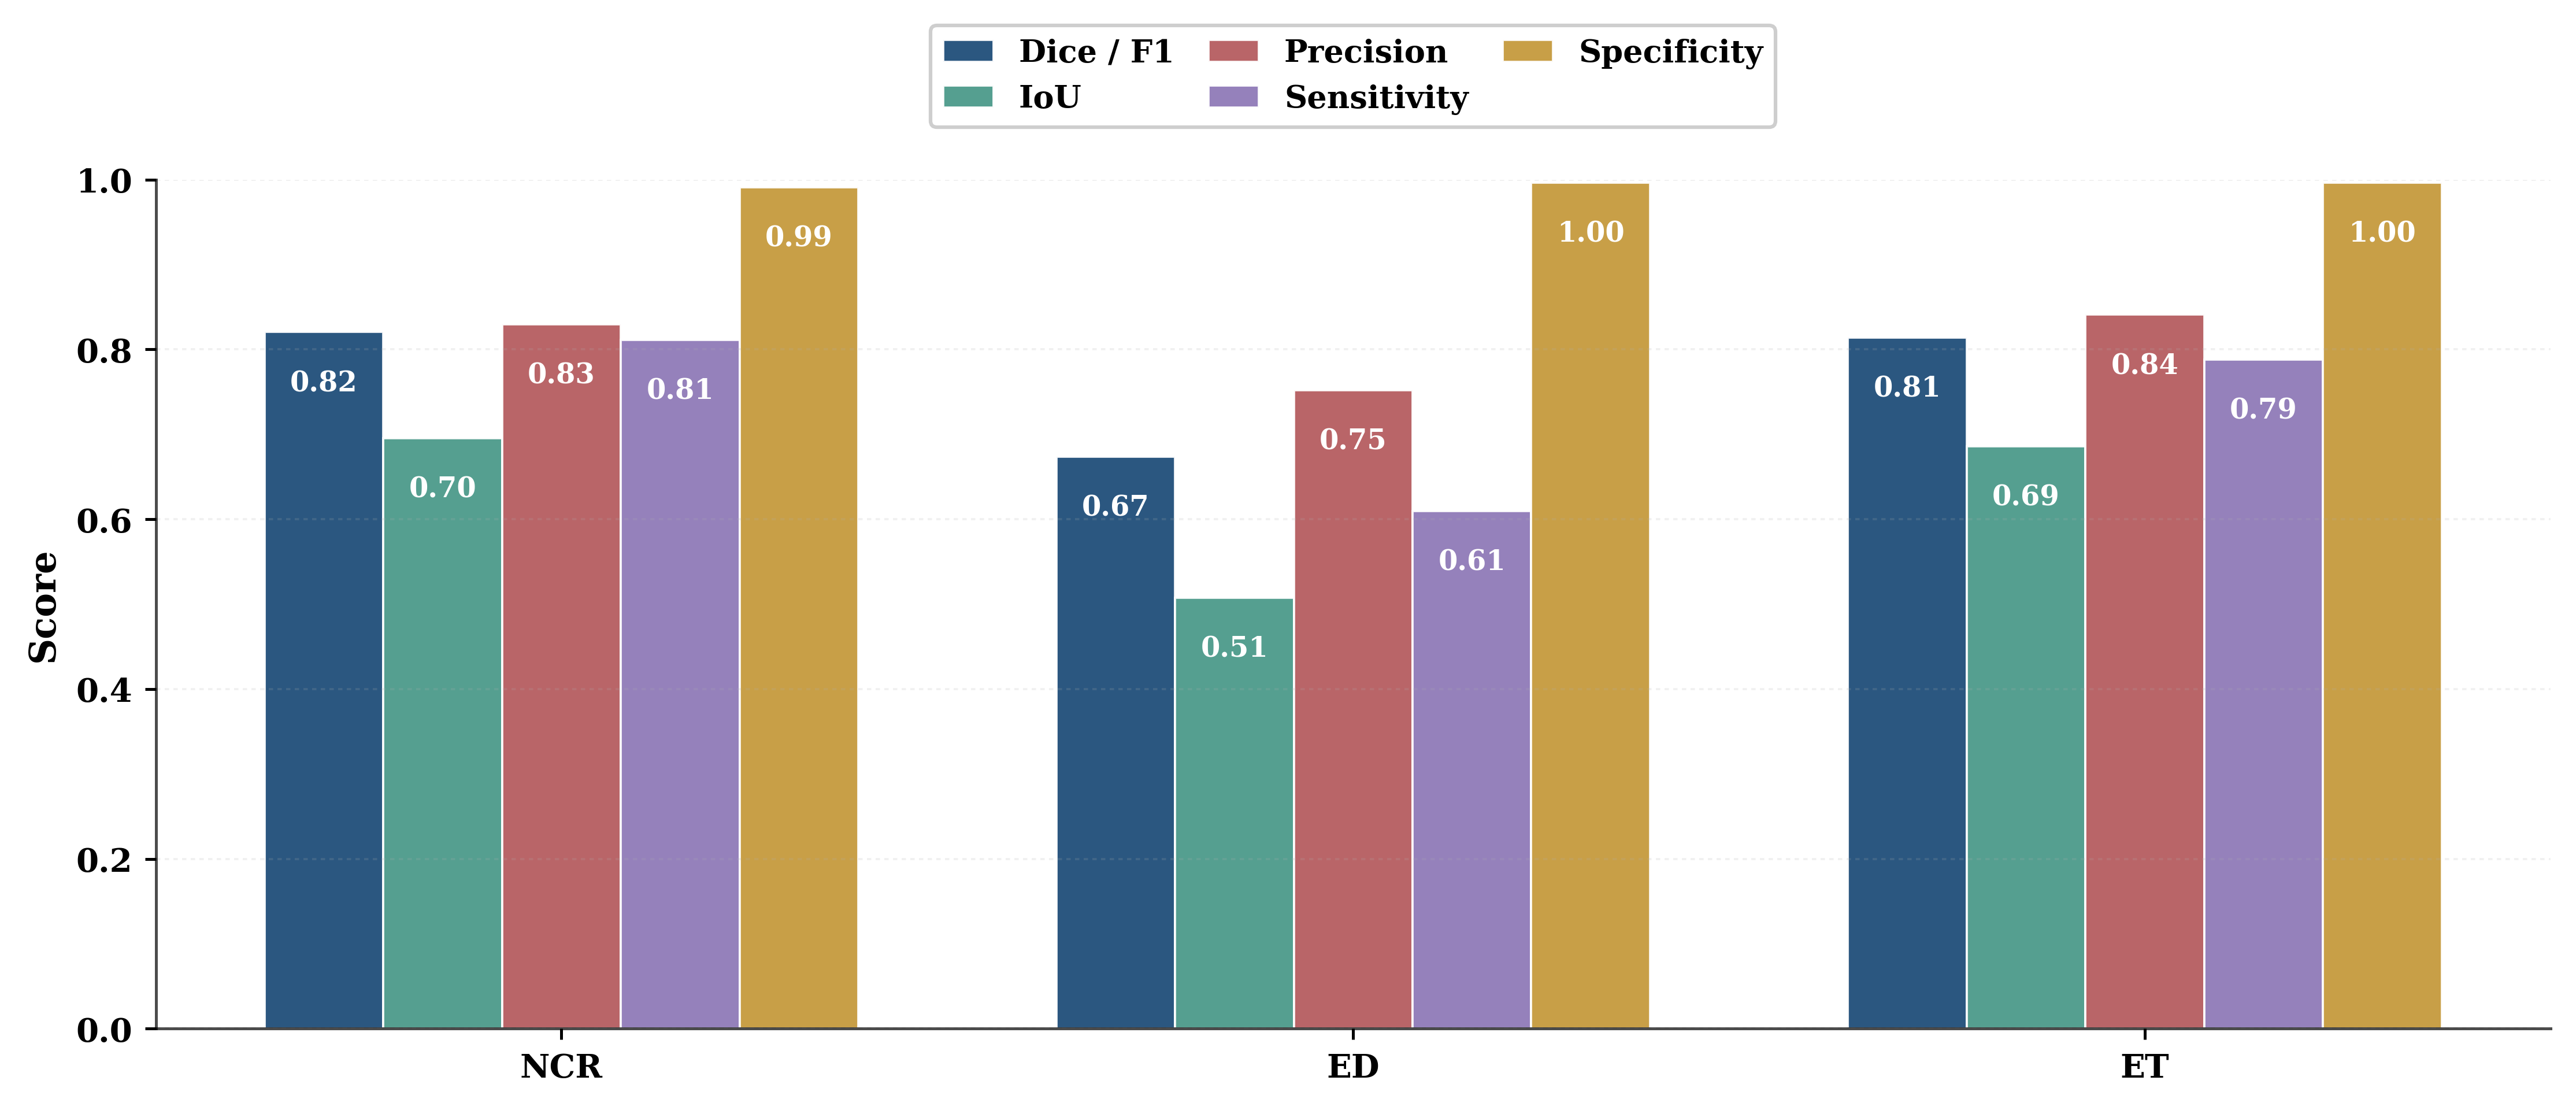
\includegraphics[width=\linewidth]{figures/eval/per_class_metrics_full.png}
\caption{Per-class performance profile of DALight-3D, reporting Dice/F1, IoU, precision, sensitivity, and specificity for NCR, ED, and ET.}
\label{fig:perclass_full}
\end{figure}

\begin{figure}[t]
\centering
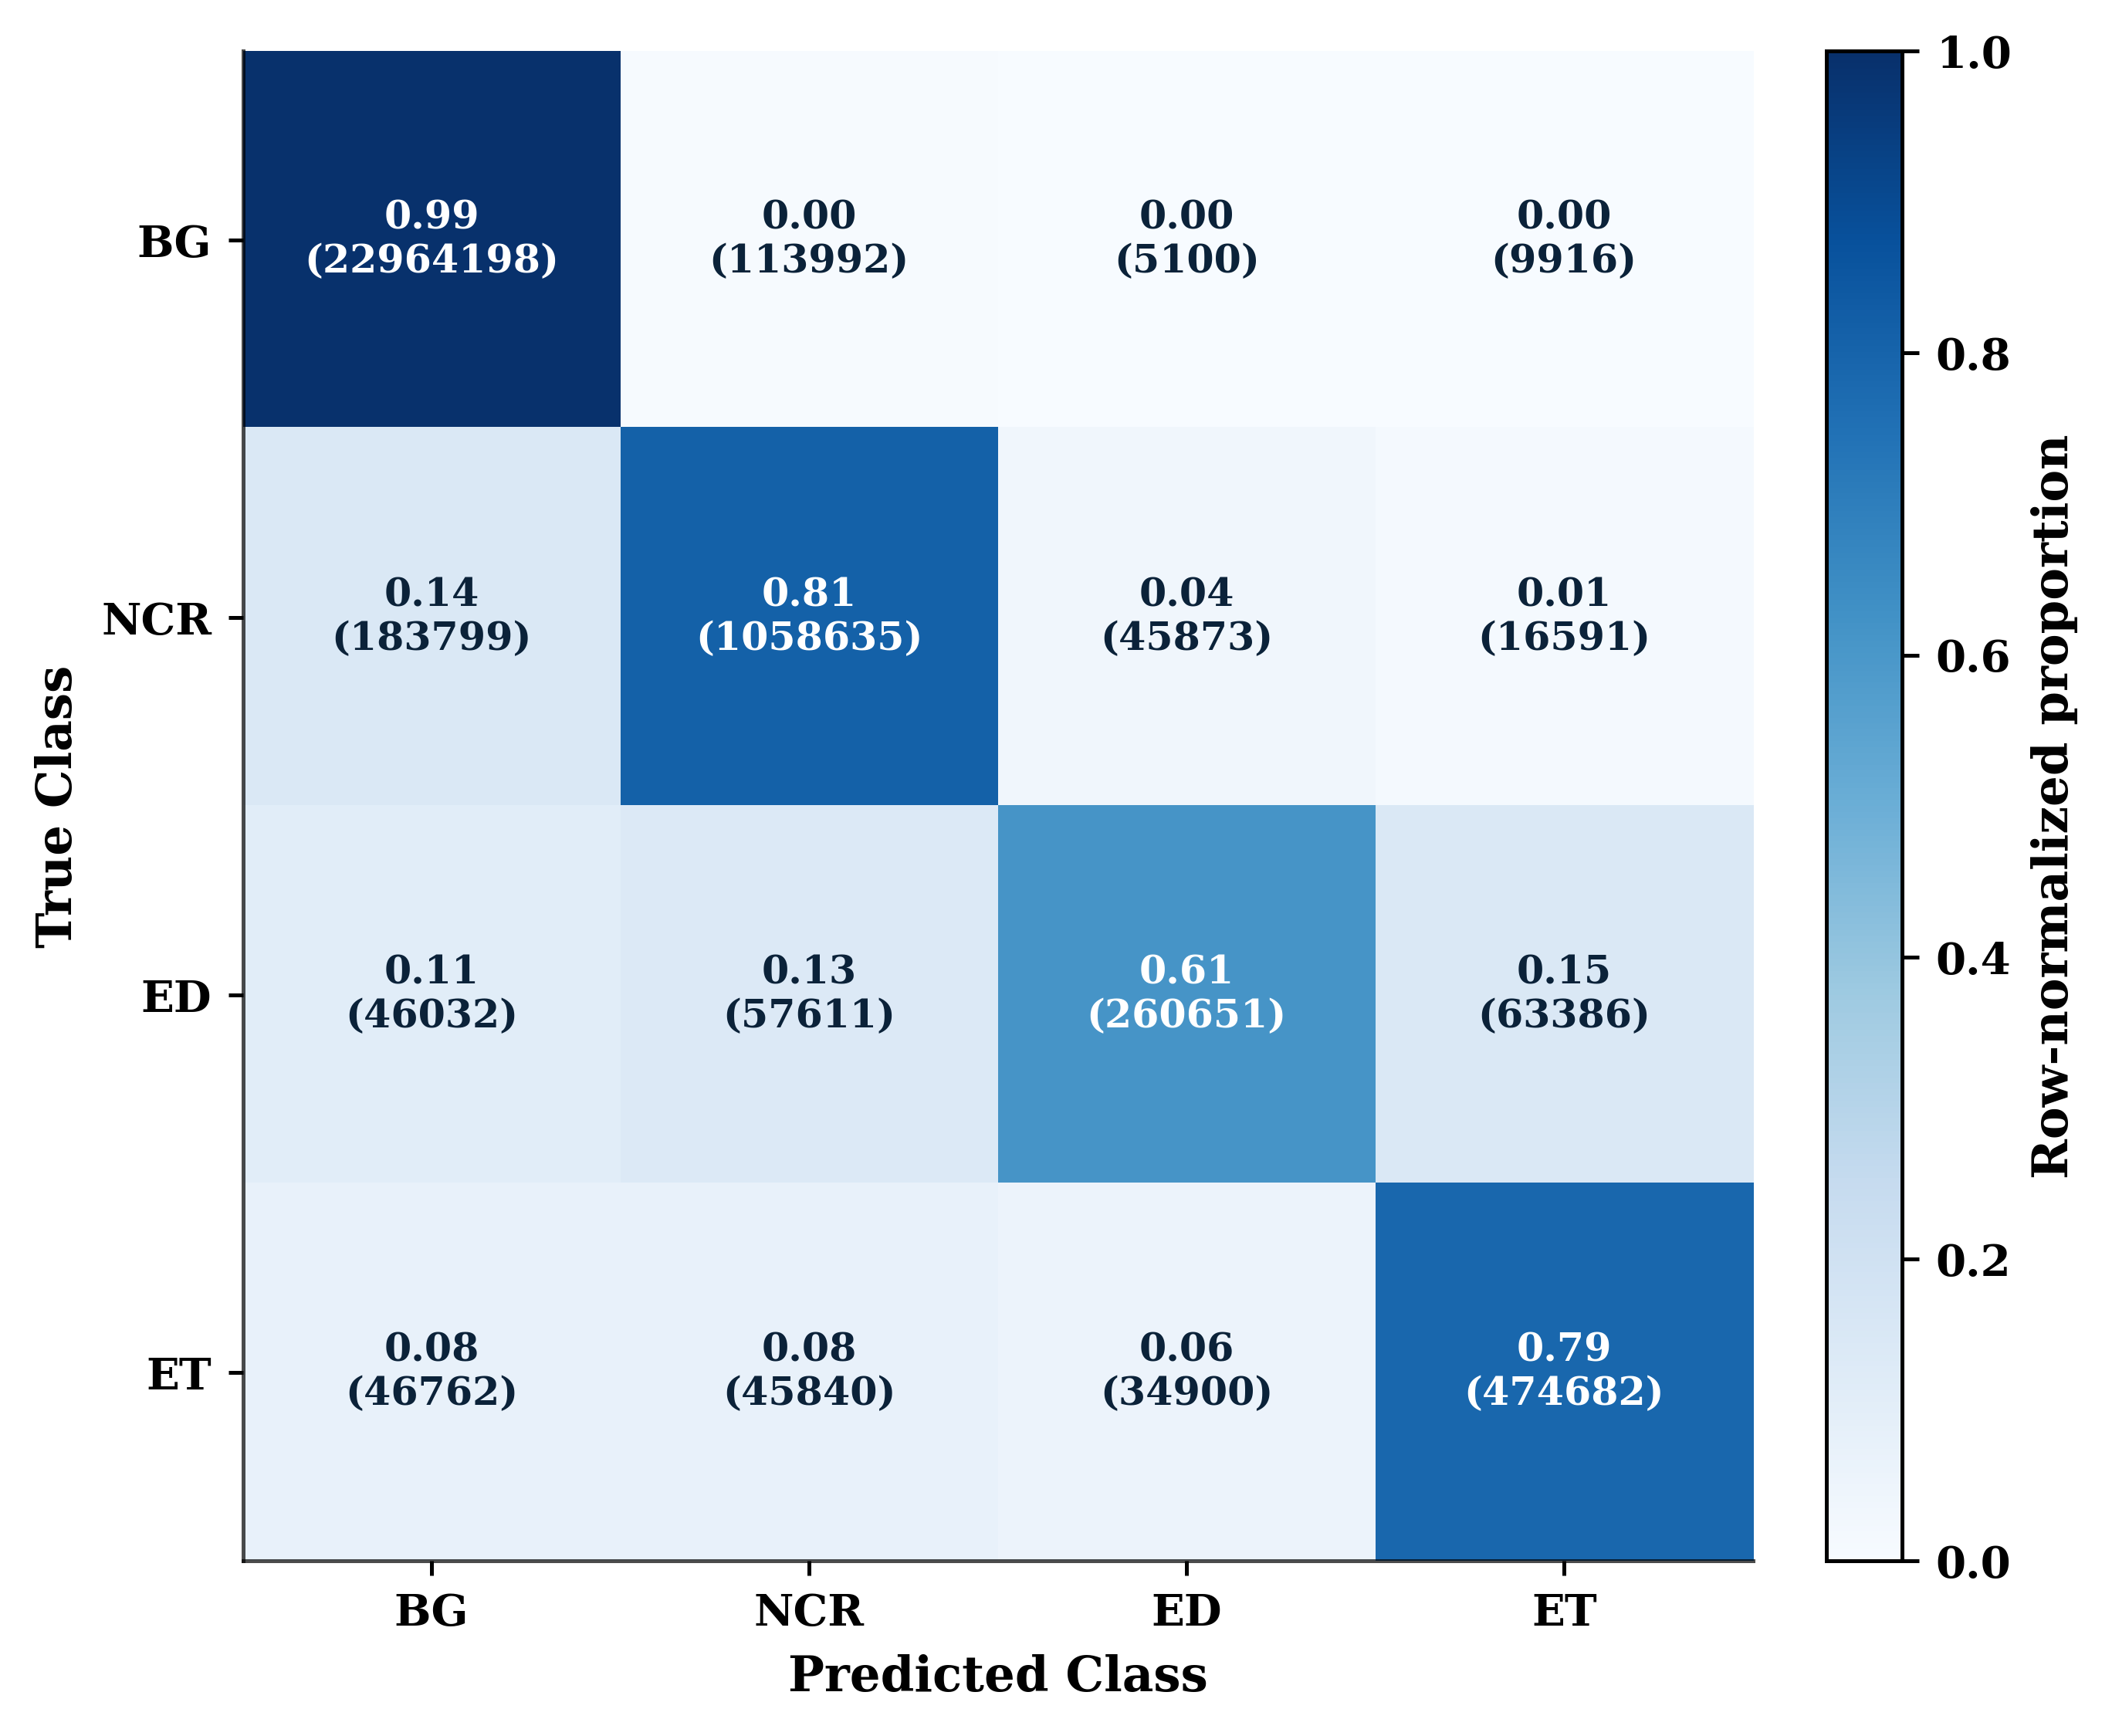
\includegraphics[width=\linewidth]{figures/eval/confusion_matrix.png}
\caption{Voxel-wise confusion matrix for DALight-3D on the validation set. The strongest confusion occurs in the edema class.}
\label{fig:confusion}
\end{figure}

\subsubsection{Calibration}

In addition to segmentation accuracy, we evaluate the reliability of the predicted probabilities through Expected Calibration Error (ECE)~\cite{guo2017calibration} using 15 bins. Calibration analysis is important because a model may achieve strong Dice while still producing poorly aligned confidence estimates. DALight-3D attains a final ECE of approximately 0.014 together with an overall voxel-wise accuracy of 0.964, indicating that its probabilities remain well behaved in addition to being discriminative. This result suggests that the model is not only segmenting accurately, but also assigning confidence in a manner that is sufficiently stable for uncertainty-aware interpretation and downstream decision-support settings.

%---------------------------------------------------------------------
\subsection{Discussion}
\label{sec:discussion}

The results indicate that the proposed design improves the accuracy--efficiency operating point of volumetric brain tumor segmentation. DALight-3D attains the highest mean Dice in the study while remaining substantially smaller than all comparison models, including the strongest baseline, Residual 3D U-Net. This outcome is important because it suggests that compactness in 3D segmentation need not come at the expense of predictive quality when efficiency-oriented design choices are introduced in a structured way. In particular, the experimental evidence is consistent with the intended role of each module: separable convolutions reduce representational cost, ScannerAwareNorm introduces explicit conditioning for scanner variability, CSA adds long-range slice-level context without the expense of full volumetric attention, and SSFB strengthens decoder-side feature fusion beyond naive skip concatenation.

The class-wise results further refine this interpretation. DALight-3D performs strongest on ET and NCR, while ED remains the most difficult region, reflecting the diffuse boundaries and lower structural specificity of edema. This pattern is consistent with prior observations in BraTS-style segmentation and suggests that the proposed architecture is especially effective when the target region exhibits stronger contrast or more compact morphology. At the same time, the low ECE indicates that the model retains useful calibration properties, which is desirable for downstream uncertainty-aware analysis and clinically oriented decision support.

Several limitations should be acknowledged. First, the current study is restricted to a single benchmark dataset and therefore does not yet establish cross-dataset generalization. Second, all models were evaluated under a relatively short 10-epoch training budget, which was sufficient to expose comparative trends but does not represent full convergence. Third, the present work emphasizes end-to-end architectural comparison rather than component-wise ablation, so the isolated contribution of SepConv, ScannerAwareNorm, CSA, and SSFB remains to be quantified more rigorously. Future work should therefore include longer training schedules, ablation studies, evaluation on external or unseen-scanner cohorts, and potentially test-time or domain-generalization strategies that further exploit the scanner-aware formulation introduced here.

%==============================================================================
\section{Conclusion}
\label{sec:conclusion}
%==============================================================================

This paper introduced \textbf{DALight-3D}, a lightweight 3D segmentation architecture for multi-modal brain tumor MRI with explicit scanner-aware feature modulation. The proposed method was motivated by a practical and still insufficiently resolved tension in volumetric medical image analysis: achieving competitive segmentation accuracy while maintaining low model complexity under heterogeneous acquisition conditions. Rather than abandoning the encoder--decoder paradigm, DALight-3D revisits it through four targeted modifications: separable 3D convolution for computational efficiency, ScannerAwareNorm for acquisition-aware feature modulation, cross-slice attention for efficient contextual reasoning, and SSFB for adaptive multi-scale fusion.

Empirically, DALight-3D achieved the strongest mean Dice among the evaluated CNN baselines on Medical Segmentation Decathlon Task01\_BrainTumour while using the fewest parameters. These findings indicate that lightweight 3D segmentation models can remain competitive when efficiency, contextual modeling, and domain sensitivity are treated as joint design objectives rather than independent add-ons. Beyond the architecture itself, the study also contributes a reproducible evaluation pipeline including parameter-aware comparison, per-class metrics, confusion analysis, and calibration assessment.

Overall, the results position DALight-3D as a compact yet effective baseline for domain-aware 3D brain tumor segmentation. Future work will focus on larger-scale validation, systematic ablation of the proposed components, and stronger robustness studies across scanners, institutions, and acquisition protocols.

%==============================================================================
\section*{References}
\bibliographystyle{ieeetr}
\bibliography{refs}

\end{document}
